\documentclass[lang=cn,10pt,onecol]{elegantbook}
\usepackage{mycommand}
% 载入quiver
\usepackage{quiver}
% Main codes
% ----------

\usetikzlibrary{shapes.symbols}	% 稍后定义 hint 环境所需

% 定义在 draftmark=true 模式下显示版本信息的指令
\usepackage[iso, english]{isodate}  % 使 \today 印出 yyyy-mm-dd
\usepackage{mathtools}

\title{代数拓扑}


\institute{呆驼调料包, 群号:679212917}
\date{Oct 1, 2024}
\version{4.3}
\bioinfo{自定义}{信息}

\extrainfo{使用 Elengantbook 模板}

\setcounter{tocdepth}{3}

\cover{cover.jpg}

% 本文档命令
\usepackage{array}
\newcommand{\ccr}[1]{\makecell{{\color{#1}\rule{1cm}{1cm}}}}
\addbibresource{引用.bib}

% 修改标题页的橙色带
% \definecolor{customcolor}{RGB}{32,178,170}
% \colorlet{coverlinecolor}{customcolor}

\begin{document}
\maketitle
\frontmatter

\tableofcontents

\mainmatter
\chapter*{序章}
\section{代数拓扑在研究什么}
\section{讨论班顺序, 主讲人以及回放查看}
\begin{enumerate}
    \item 范畴论回顾, 方便的空间范畴; 主讲人: 刘欧; 回放:\href{https://www.bilibili.com/video/BV1thxEeRE6h/?spm_id_from=333.999.0.0}{Lecture 1.1}, .
    \item 待续
\end{enumerate}

\chapter{范畴论回顾, 方便的空间范畴}
\begin{introduction}
    \item \textbf{范畴论} 是一门数学分支, 最开始由 MacLane 引入以解释自然变换的``自然性''.请读者回忆有限维向量空间 $V$ 与其双重对偶 $(V^{\lor})^{\lor}$ 的自然同构 $\ev_V : V \simeq (V^{\lor})^{\lor}$, 在线性代数中, 我们称该同构是``自然的'', 或 ``典范的'', 以 $\ev_V$ 为例, 一般而言, 可以如下来理解自然性
    
\begin{enumerate}
    \item 它不依赖于基的选取, 事实上, 可以直接写下它的公式 $\ev_V(v) = \left<-,v\right>\colon V^{\lor} \to F$, 这并不需要任意诸如有序基的辅助信息.
    \item 它与线性映射的结构是兼容的, 即
    \[\begin{tikzcd}
	V & W \\
	{V^{\lor \lor}} & {W^{\lor \lor}}
	\arrow["T", from=1-1, to=1-2]
	\arrow["{\ev_V}"', from=1-1, to=2-1]
	\arrow["{\ev_W}", from=1-2, to=2-2]
	\arrow["{T^{\lor \lor}}"', from=2-1, to=2-2]
    \end{tikzcd}\]
\end{enumerate}

\item 范畴论的原理是将不同数学分支的数学理论抽象出来, 只保留两种信息: 数学对象, 以及其间态射(我们所关心的箭头, 或者说是相容的箭头, 例如在我们关心拓扑空间时, 所考虑的箭头即为连续映射, 在关心概形时, 所考虑的箭头往往为概形间的态射). 由此我们可以解释自然或者典范.\\
在考虑从结构 $A$ 中得到结构 $B$ 的信息时(或者说从范畴 $\cal{C}$ 中得到范畴 $\cal{D}$ 的信息, 比方说你考虑带点拓扑空间 $(E,e)$ 的基本群 $\pi_1((E,e))$ 时), 我们就需要用到函子的概念, 上述例子给出了一个函子 $\cate{Top}_{\star} \to \cate{Grp}$(例~\ref{例:范畴}), 更为经典的使用函子的例子是 Brouwer 不动点的证明, 可见定理~\ref{定理:Brouwer}.\\
当然, 函子可能具有一些诸如伴随, 保(余)极限, 可表等性质具体内容我们将在后文进行讨论.\\

\item 在一切开始之前, 我们还需要进行一个观察:
在讨论群的时候, 我们经常认为同构的群是一致的; 在讨论拓扑空间的时候, 我们经常认为同胚的拓扑空间就是一致的.
所以同构/同胚是一种在对应结构中所适用的等号(在对应的代数结构中它往往比严格相等更加有用).因此在范畴论中, 我们自然而然的提出一个朴素观点: \textbf{以同构代替严格等式}.\footnote{当然, 在类型论中, 直接在类型里提出相等类型的概念, 具体分为赋值相等和命题相等, 在此不做过多探讨, 感兴趣的读者请参看类型论相关资料.}

\item 考虑到讨论班参加成员均为初学者, 本文将不会过多讨论 Grothendieck 宇宙的内容, 本文选定一个 Grothendieck 宇宙 $\mathcal{U}$ 若无额外说明, 我们统一认定为小范畴, 即 $\Obj$ 与 $\Mor$ 均为 $\cal{U}$-小集合(即落在 $\cal{U}$ 内)的情况.
\end{introduction}

\begin{flushright}\begin{minipage}{0.3 \textwidth}
	\begin{tabular}{c}
		{作者: \kaishu 刘欧} \\
		2024.9  
	\end{tabular}
\end{minipage}\end{flushright}
\section{范畴, 函子, 自然变换}

本节来介绍基础的范畴与函子概念
\subsection{范畴}
粗略来说, 范畴就是一些点与其间的箭头所构成的结构,其具体定义如下:
\begin{definition}[(1-)范畴]\label{定义:1-范畴}
    一个(1-)范畴 $\cal{C}$ 系指以下信息:
    \begin{enumerate}
        \item 集合 $\Obj(\cal{C})$ , 其内元素称作 $\cal{C}$ 的\textbf{对象}.
        \item 对任意 $x, y \in \Obj (\mathcal{C})$, 有一个集合$\Hom_{\mathcal{C}} (x, y)$, 其元素称为从 $x$ 到 $y$ 的\textbf{态射}.
        \item 对任意 $x \in \Obj (\mathcal{C})$,
            有一个元素
            \[
                \identity_x \in \Hom_{\mathcal{C}} (x, x),
            \]
            称为 $x$ 到自身的\textbf{恒等态射}.
        \item 对任意 $x, y, z \in \Obj (\mathcal{C})$,
            有一个映射
            \begin{align*}
                \circ \colon
                \Hom_{\mathcal{C}} (x, y) \times \Hom_{\mathcal{C}} (y, z)
                & \to \Hom_{\mathcal{C}} (x, z), \\
                (f, g) & \mapsto g \circ f,
            \end{align*}
            称为\textbf{复合},
    \end{enumerate}
    并且满足以下两条公理
     \begin{itemize}
        \item
            (\textbf{单位律})
            对任意 $x, y \in \operatorname{Ob} (\mathcal{C})$,
            及任意 $f \in \mathcal{C} (x, y)$, 有
            \[
                \identity_y \circ f = f = f \circ \identity_x.
            \]
        \item
            (\textbf{结合律})
            对任意 $x, y, z, w \in \operatorname{Ob} (\mathcal{C})$,
            及任意 $f \in \mathcal{C} (x, y)$,
            $g \in \mathcal{C} (y, z)$, 
            $h \in \mathcal{C} (z, w)$, 有
            \[
                (h \circ g) \circ f = h \circ (g \circ f),
            \]
            故可记之为 $h \circ g \circ f$, 而不产生歧义.
    \end{itemize}
\end{definition}
\begin{remark}\label{注记:范畴}
    我们常常使用以下记号:
\begin{itemize}
    \item
        如果 $x \in \operatorname{Ob} (\mathcal{C})$,
        我们简记为 $x \in \mathcal{C}$.

    \item
        如果 $f \in \Hom_{\mathcal{C}} (x, y)$,
        我们也记 $f \colon x \to y$, 或者 $x \xrightarrow{f} y$.

    \item
        $\mathcal{C}$ 中所有态射构成的类常常记为
        $\operatorname{Mor} (\mathcal{C})$, 此时具有一对典范映射 
        \begin{tikzcd}
	{\Mor(\cal{C})} & {\Obj(\cal{C})}
	\arrow["t"', shift right, from=1-1, to=1-2]
	\arrow["s", shift left, from=1-1, to=1-2]
        \end{tikzcd}
        分别表示态射的\textbf{来源}和\textbf{目标}.
    \item 图表加箭头是讨论范畴的方便语言. 其中最常用的是\textbf{交换图表}的概念, ``交换'' 指态射合成后的结果相等,就是说图表中链接同一始末点组的道路给出相同的作用效果, 例如以下二则图表
    \[\begin{tikzcd}
	x & y \\
	& z
	\arrow["f", from=1-1, to=1-2]
	\arrow["{h}"', from=1-1, to=2-2]
	\arrow["g", from=1-2, to=2-2]
    \end{tikzcd}\quad
    \begin{tikzcd}
	x & y \\
	w & z
	\arrow["f", from=1-1, to=1-2]
	\arrow["u"', from=1-1, to=2-1]
	\arrow["g", from=1-2, to=2-2]
	\arrow["v"', from=2-1, to=2-2]
    \end{tikzcd}\]
    的交换性分别再说 $g\circ f = h$ 以及 $v\circ u = g\circ f$.\footnote{事实上在高阶范畴论中, 图表交换是信息而非性质.}
\end{itemize}
\end{remark}

事实上, 在这一步我们没有做什么不平凡的举动, 为方便读者理解, 我们给出以下例子
\begin{example}\label{例:范畴}
    \begin{enumerate}
        \item 当我们关心某一类数学对象的全体时, 可以取它们构成的范畴, 此时态射即为数学结构所容许的映射,或者说保持数学结构的映射, 例如
        \begin{itemize}
            \item 所有$\cal{U}$-小集合及其间映射构成范畴 $\cate{Set}$.
            \item 所有$\cal{U}$-小群及其间群同态构成的范畴 $\cate{Grp}$.
            \item 域 $\Bbbk$ 上全体向量空间及其间线性映射所构成的范畴 $\cate{Vect}({\Bbbk})$.
            \item 拓扑空间及其间连续映射构成范畴 $\cate{Top}$.
            \item 所有光滑流形及其间光滑映射构成范畴 $\cate{Mani}$.
            \item 可测空间及其间可测函数构成范畴 $\cate{Meas}$, 但是这一空间事实上缺少了很多信息(比如说零测的选取), 所以难堪大用.
            \item $R$-模上的链复形及其间链映射构成范畴 $\cate{\Chain_R}$.
            \item 全体概形及其间态射构成范畴 $\cate{Sch}$.
        \end{itemize}
        \item 我们也可以将集合 $S$ 升级为对应的范畴, 记作 $\cate{Disc}(S)$, 其对象集为 $S$ 而态射只有恒等态射.
        \item(子范畴) 有时候我们会在原范畴 $\cal{C}$ 中取出一部分对象($\Obj(\cal{C}')\subset \Obj(\cal{C})$)与态射(当然取出的态射$f$ 需要保证 $s(f), t(f) \in \Obj(\cal{C}')$) 所构成新范畴, 并且其它一切性质(即恒等态射, 结合律等)都继承自原范畴, 我们把这一新结构称为$\cal{C}$ 的子范畴. 当取出的态射正好为取出对象之间全体态射时, 我们把子范畴称为全(或者满)子范畴, 后面将看到这作为嵌入函子确实是全的.
        \item 取 $\Bbbk$ 上全体有限维向量空间所构成的范畴 $\cate{Vect}_{f}(\Bbbk)$, 容易发现其为 $\cate{Vect}(\Bbbk)$ 的全子范畴.
        \item 带点拓扑空间构成的范畴 $\cate{Top}_{\star}$, 其对象为所有的 $(E,e)$, 其中 $e \in E$ 称为基点. 从 $(X,x)$ 到 $(Y,y)$ 的态射为保持基点的连续映射, 即使得 $f(x) = y$ 的连续映射 $f:X \to Y$.
        \item 全体 Abel 群构成的范畴 $\cate{Ab}$, 它是 $\cate{Grp}$ 的全子范畴.
        \item(这两个例子可以不看XD) 以测度空间作为对象, 对于其间可测映射取以几乎处处相等(即不相等的地方在零测集内)作为等价关系的等价类(还需要保证可测映射关于零测集的原像为零测集), 可以得到范畴 $\cate{Measure}$, 但是这个范畴的信息太多, 每个对象都带有一个特定的测度, 这会导致我们做出一些不典范的选择.
        \item 一般而言, 我们考虑强化可测空间, 它是三元组 $(X,M,N)$, 其中 $M$ 为 $\sigma$-代数而 $N$ 为其表示零测部分所构成的 $\sigma$-理想, 对于可测函数 $f : (X,M,N) \to (Y,M',N')$ , 若对于任意 $n\in N'$, 都有 $f^{-1}(n) \in N$, 则称 $f$ 为保零测的.此外, 对于 $f,g : (X,M,N) \to (Y,M',N')$, 若对于任意 $m\in M'$ 有 $f^{-1}m'\oplus g^{-1}m'\in N$, 则称它们几乎处处弱相等.
        从而我们得到以强化可测空间作为对象, 保零测的可测函数集商去几乎处处弱相等的可测函数作为态射集所得到的范畴, 记为$\cate{EMS}$, 更加详细的内容可见\href{https://ncatlab.org/nlab/show/categories+of+measure+theory}{nlab}.
        \item 我们可以给出全体(小)范畴所构成的范畴 $\cate{Cat}$, 但后文我们将发现, 仅仅视其为 1-范畴是不自然的, 因为这样会损失自然变换(即2-态射)的信息, 它应该被视为一种 2-范畴, 详见无穷范畴笔记附录.
    \end{enumerate}
\end{example}
在谈论函子之前, 请容许我们对于范畴进行多一点点的观察, 就是考虑范畴内态射的性质.显然的, 我们可以将单满性以及同构移入范畴之中.
\begin{definition}
    设 $x,y$ 为范畴 $\cal{C}$ 中的对象, $f:x \to y$ 为态射.则
    \begin{itemize}
        \item 称 $f$ 为\textbf{单态射}, 如果对任意 $Z\in \cal{C}$ 以及一对态射 $g,h : Z \to X$ 都有 $fg = fh \Leftrightarrow g=h$(左消去律);
        \item 称 $f$ 为\textbf{满态射}, 如果对任意 $Z \in \cal{C}$ 以及一对态射 $g,h : Y \to Z$ 都有 $gf = hf \Leftrightarrow g=h$(右消去律);
    \end{itemize}
    如果存在 $g$ 使得 $gf = \identity_X$ 则称 $f$ 左可逆而 $g$ 为其左逆; 类似地, $fg = \identity_Y$ 则称 $f$ 右可逆而 $g$ 为其右逆; 左可逆又右可逆的态射称为同构.
\end{definition}
\begin{definition}[子对象]\label{定义-子对象}
    在一般的范畴中, 称指向 $X$ 的单态射 $U\to X$ 的同构类为 $X$ 的子对象, 其中单态射的同构是指形如
    \[\begin{tikzcd}
	U \\
	&& X \\
	{\tilde{U}}
	\arrow[hook, from=1-1, to=2-3]
	\arrow["\simeq"', shift right, from=1-1, to=3-1]
	\arrow[shift right, from=3-1, to=1-1]
	\arrow[hook, from=3-1, to=2-3]
    \end{tikzcd}\]
    的交换图. $X$ 的子对象构成偏序集 $\Sub_{\cal{C}}(X)$.
\end{definition}
显然地,左可逆蕴含单而右可逆蕴含满, 一个态射是同构当且仅当它左右均可逆.但是一个态射$f: X \to Y$即单又满并不代表其为同构, 这是缘于它不一定是严格态射($\Image(f)\rightiso \op{coim}(f)$\footnote{事实上, 可以说明满态射相当于说 $\Image(f) \rightiso Y$, 而单态射相当于说 $X \rightiso \op{coim}(f)$.},但很可惜, 我们估计不会讲), 这也是在同调代数中, 我们一般考虑 Abel 范畴(Abel 范畴 $\cal{A}$ 为加性范畴, 所有态射皆有核与余核且严格.).
而后, 我们就可以给出一个新的例子
\begin{definition}[群胚]
    若一个范畴 $\cal{C}$ 的所有态射均可逆, 则称其为\textbf{群胚}, 群胚所构成的范畴记为 $\cate{Groupoid}$.
\end{definition}
\begin{example}
    群就是只有一个对象, 且态射为群元素的群胚, 将群 $G$ 视为群胚的过程叫做群的胚化, 记为 $\underline{G}$.
\end{example}
事实上, 群胚是一个 (1,0)-范畴\footnote{所谓(m,n)-范畴是指 $k>n$ 的态射皆可逆的 $m$-范畴}, 并且是集合的推广. 如果只考虑 1-范畴, 则可以将群胚视为群的推广.\\
事实上, 群胚是更贴合于拓扑空间结构的 1-范畴, 正如 $\infty$-群胚(或者说 Kan 复形)是贴合于拓扑空间结构的单纯集一般, 我们可以很自然地从拓扑空间中取出群胚(当然,只是从同伦的角度来看, 这是从拓扑空间造出 1-范畴的典范手段), 称为基本群胚.
\begin{example}
    对于拓扑空间 $E$ ,其\textbf{基本群胚} $\Pi_{1}(E)$ 定义为如下范畴:
    \begin{itemize}
        \item $\Obj(\Pi_1(E)) = E$.
        \item $\Hom_{\Pi_1(E)}(x_0,x_1) = $从 $x_0$ 到 $x_1$ 的道路类.
        \item $\identity_{x_0} = [c_{x_0}]$ 其中右侧表示在 $x_0$ 处的常值道路.
    \end{itemize}
\end{example}
关于基本群胚的细节探讨我们放在后文进行, 在这里我们只留下一个悬念, 即考虑基本群胚的时候我们实际上把道路之间的同伦商去了, 这会使我们损失一些信息(正如我们在考虑复形 $\chain(\cal{A})$ 的同伦范畴 $\cate{K}(\cal{A})$ 时, 我们商去了零伦, 这会导致后来局部化时出现问题, 即在定义导出范畴时好三角无法精确到唯一同构, 三角范畴缺少核与余核, 导出函子无法简单刻画等问题), 所以我们不应该商去这些同伦(那么同伦间的同伦是否应该商去呢?), 而应该保持这些``高阶''的态射(那又该怎样合理的构造呢?), 在此我们先装聋作哑把 1-范畴学懂, 至于考虑高阶态射后的 $\infty$-范畴留待读者自行探索.\\
此外, 范畴具有着对偶构造(不过是把态射倒置)\footnote{在高阶范畴上, 会出现不止一种对偶结构,即不仅仅可倒置1-态射,还可以倒置高阶态射.}, 即反范畴, 其具体定义如下:
\begin{definition}
    对于任意范畴 $\cal{C}$, 定义其反范畴 $\cal{C}^{\opposite}$ 如下:
    \begin{itemize}
        \item $\Obj(\cal{C}^{\opposite}) = \Obj(\cal{C})$, 对于 $X\in \cal{C}$, 记其在反范畴中的对应为 $X^{\opposite}$.
        \item 对于任意对象 $X,Y$, $\Hom_{\cal{C}^{\opposite}}(X^{\opposite},Y^{\opposite}) \coloneqq \Hom_{\cal{C}}(Y,X)$.
        \item 反范畴中的态射合成 $\circ$ 定义为 $\cal{C}$ 中的反向合成.
        \item 恒等映射同 $\cal{C}$.
    \end{itemize}
\end{definition}
后文我们将看到对偶构造 $(-)^{\opposite}$ 构成函子.
\subsection{函子}
现在我们来讲一下函子, 粗略地说, 函子也是一种态射, 它不过是保持范畴结构的态射而已, 由于范畴具有对象集与态射集两种结构, 因此函子也理当从这两种结构上考虑, 此外函子并不需要带有更多的信息, 只需要保证范畴公理(即定义~\ref{定义:1-范畴})的照常运作即可.
\begin{definition}[函子]
    设 $\cal{D}$, $\cal{C}$ 为范畴, 一个函子 $F: \cal{C} \to \cal{D}$ 系指以下信息:
    \begin{enumerate}
        \item 对象集之间的映射 $F: \Obj(\cal{C}) \to \Obj(\cal{D})$.
        \item 态射之间的映射 $\Hom_{\cal{C}}(x,y)\to \Hom_{\cal{D}}(F(x),F(y))$.
    \end{enumerate}
    需要满足以下公理:
    \begin{itemize}
        \item 对每个 $x\in \Obj(\cal{C})$ 都有
        \[
        F(\identity_x) = \identity_{F(x)}.
        \]
        \item 它将 $\cal{C}$ 中如下交换图映为 $\cal{D}$ 中的交换图
        \[\begin{tikzcd}
	x & y \\
	& z
	\arrow["f", from=1-1, to=1-2]
	\arrow["{g\circ f}"', from=1-1, to=2-2]
	\arrow["g", from=1-2, to=2-2]
       \end{tikzcd} \Rightarrow 
       \begin{tikzcd}
	{F(x)} & {F(y)} \\
	& {F(z)}
	\arrow["{F(f)}", from=1-1, to=1-2]
	\arrow["{F(g)\circ F(f)}"', from=1-1, to=2-2]
	\arrow["{F(g)}", from=1-2, to=2-2]
        \end{tikzcd}\]
    \end{itemize}
\end{definition}
而后我们给出一些例子以资体会
\begin{example}
    \begin{enumerate}
    \item 每个范畴 $\cal{C}$ 都有到自身的恒等函子, 记为 $\identity_{\cal{C}}$.
    \item 前文所提到的子范畴 $\cal{C}'$ 到原范畴 $\cal{C}$ 的含入可以构成函子, 称其为包含函子, 记作 $\iota : \cal{C}' \hookrightarrow \cal{C}$.
    \item 对于范畴的范畴 $\cate{Cat}$ 可以定义对偶构造 $(-)^{\opposite}: \cate{Cat} \to \cate{Cat}$, 它将范畴 $\cal{C}$ 映为其反范畴 $\cal{C}^{\opposite}$, 范畴间的函子映为反范畴间的对应函子. 不难发现在 1-范畴语境下 $((-)^{\opposite})^{\opposite} = \identity_{\cate{Cat}}$.
    \item 考虑域 $\Bbbk$ 上的向量空间范畴 $\cate{Vect}(\Bbbk)$, 回忆其对偶空间定义为
    \[
    V^{\lor} \coloneqq \Hom_{\Bbbk}(V,\Bbbk) = \{\Bbbk\,\text{-线性映射}\, V \to \Bbbk\}
    \]
    对于任一线性映射 $f: V_1 \to V_2$, 它通过以下图表的方式诱导对偶空间的反向线性映射(即转置映射, 其作用效果为复合上 $f$, 容易发现在有限维取基用矩阵表出后即为矩阵转置)
    \[\begin{tikzcd}
	& {V_2^{\lor}=\Hom_{\cate{Vect}_{\Bbbk}}(V_2,\Bbbk)} \\
	{V_1} & \Bbbk \\
	{V_2} & {V_1^{\lor}=\Hom_{\cate{Vect}_{\Bbbk}}(V_1,\Bbbk)}
	\arrow[""{name=0, anchor=center, inner sep=0}, "{f^{\lor}(a) = a\circ f}", from=2-1, to=2-2]
	\arrow["f"', from=2-1, to=3-1]
	\arrow[""{name=1, anchor=center, inner sep=0}, "a"', from=3-1, to=2-2]
	\arrow["{f^{\lor}}"', shift right=5, from=3-2, to=1-2]
	\arrow["\in"{marking, allow upside down}, draw=none, from=0, to=1-2]
	\arrow[shorten <=2pt, shorten >=2pt, maps to, from=1, to=0]
	\arrow["\in"{marking, allow upside down}, draw=none, from=1, to=3-2]
    \end{tikzcd}\]
    具体写出即为
    \begin{align*}
        f^{\lor} : V_2^{\lor} = \Hom_{\cate{Vect}(\Bbbk)}(V_2,\Bbbk) &\to V_1^{\lor} = \Hom_{\cate{Vect}(\Bbbk)}(V_1,\Bbbk),\\
        [a: V_2 \to \Bbbk] &\mapsto  a \circ f
    \end{align*}
    易见 $D: V \mapsto V^{\lor}$, $f\mapsto f^{\lor}$ 定义了函子 $D: \cate{Vect}(\Bbbk)^{\opposite} \to \cate{Vect}(\Bbbk)$, 我们可以再取一次对偶并且复合后得到函子 $DD^{\opposite} : \cate{Vect}(\Bbbk) \to \cate{Vect}(\Bbbk)$. 分别称 $D$ 和 $DD^{\opposite}$ 为对偶和双对偶函子.
    \item 对于带点拓扑空间 $(E,e)\in \cate{Top}_{\star}$, 指定其基本群 $\pi_1(E,e)$ 就给出函子 $\cate{Top}_{\star} \to \cate{Grp}$, 若指定大于等于 2 的高阶同伦群则给出函子 $\cate{Top}_{\star} \to \cate{Ab}$, 此外, 空间的(某种)同调群 $X \mapsto H_n(X;\Z)$ 给出一族函子 $H_n: \cate{Top} \to \cate{Ab}$. 而上同调群给出函子 $H^n : \cate{Top}^{\opposite} \to \cate{Ab}$.
    \item 从拓扑空间到其基本群胚给出函子 $\Pi:\cate{Top} \to \cate{Groupoid}$, 群的胚化给出函子 $\underline{(-)}: \cate{Grp} \to \cate{Groupoid}$.
    \end{enumerate}
\end{example}
由于函子作用于两个层面, 并且回忆到我们先前所提到过的范畴论的哲学原理, 我们可以给出函子作为映射的部分性质, 由于范畴论以同构代替严格等式, 因此在对象上我们不苛求严格相等, 而在态射上, 我们以 $\Hom$-集为主体进行考虑,自然需要考虑单满性.
\begin{definition}
    对于函子 $F: \cal{C} \to \cal{C}'$,
    \begin{enumerate}
        \item 称 $F$ 为本质满的, 若 $\cal{C}$ 中的任一对象都同构于某个 $F(x)$;
        \item 称 $F$ 是忠实的, 若对所有的 $x,y \in \cal{C}'$ 映射 $\Hom_{\cal{C}'}(x,y) \to \Hom_{\cal{C}}(Fx,Fy)$均为单射.
        \item 若上述映射对于所有 $x,y \in \cal{C}'$ 均为满射, 则称 $F$ 是全的.
    \end{enumerate}
\end{definition}
\begin{exercise}
    观察上述例子, 说明哪些函子是本质满的, 哪些函子是全的, 哪些函子是忠实的.
\end{exercise}
到函子这一层就已经可以进行一些粗浅的应用, 典型案例就是 Brouwer 不动点定理的证明.
\begin{theorem}[Brouwer 不动点定理]\label{定理:Brouwer}
    设 $D^n$ 是 Euclid 空间中的单位球体,
    则对任意连续映射 $f \colon D^n \to D^n$,
    存在 $x \in D^n$, 使得 $f(x) = x$.
\end{theorem}
\begin{proof}
    如不然, 记 $S^{n-1}$ 为单位球面, 则映射
    \[
        \pi \colon D^n \to S^{n-1}, \quad
        x \mapsto \text{射线}\ f(x) \to x\ \text{与}\ S^{n-1}\ \text{的交点}
    \]
    与含入映射 $i \colon S^{n-1} \to D^n$ 之复合为恒等映射.
    于是它对应的 $n-1$ 阶约化同调群映射 
    \[
        \widetilde H_{n-1}(S^{n-1}) \to
        \widetilde H_{n-1}(D^n) \to
        \widetilde H_{n-1}(S^{n-1})
    \]
    之复合是恒等映射. 但 $\widetilde H_{n-1}(D^n) = 0$, 
    $\widetilde H_{n-1}(S^{n-1}) = \Z$, 矛盾.
\end{proof}
当然你也可以使用基本群进行证明维数为 2的情况, 因为你可以根据直观显然得到 $\pi_1(D^2) = 0$ 而 $\pi_1(S^1) = \Z$.
\subsection{自然变换}
现在我们已经给出了函子的定义, 那么我们其实可以观察到在引言中我们所说的线性空间与双对偶空间的交换图表能够改写如下
\[\begin{tikzcd}
	V & W \\
	{DD^{\opposite}V} & {DD^{\opposite}W}
	\arrow["f", from=1-1, to=1-2]
	\arrow["\ev"', from=1-1, to=2-1]
	\arrow["\ev", from=1-2, to=2-2]
	\arrow["{DD^{\opposite}(f)}", from=2-1, to=2-2]
\end{tikzcd}\]
可以看出这自然地勾连了函子 $\identity_{\cate{Vect}_f(\Bbbk)}$ 以及双对偶函子 $DD^{\opposite}$. 本节中我们来仔细探讨这一性质, 不难发现, 这一性质恰好可以视为函子间的态射(保持了函子的结构), 因此自然性也称为函子性.
\begin{definition}[自然变换,或函子间的态射]
    设 $\cal{C}$, $\cal{D}$ 为范畴, $F,G:\cal{C} \to D$ 为函子, 从 $F$ 到 $G$ 的\textbf{自然变换} $\alpha$ 通常记为
    \[
    \alpha : F \Rightarrow G,
    \]
    由以下信息构成:
    \begin{itemize}
        \item 对每个 $x\in \cal{C}$, 都有 $\cal{D}$ 中态射 $\alpha_x : F(x) \to G(x)$.
    \end{itemize}
    满足以下相容性(自然性)条件:对于 $\cal{C}$ 中任一态射 $f:x \to y$, 有 交换图
    \[\begin{tikzcd}
	{F(x)} & {F(y)} \\
	{G(x)} & {G(y)}
	\arrow["{F(f)}", from=1-1, to=1-2]
	\arrow["{\alpha_x}"', from=1-1, to=2-1]
	\arrow["{\alpha_y}", from=1-2, to=2-2]
	\arrow["{G(f)}"', from=2-1, to=2-2]
    \end{tikzcd}\]
\end{definition}
可以以2-胞腔的形式写为
\[\begin{tikzcd}
	{\cal{C}} && {\cal{D}}
	\arrow[""{name=0, anchor=center, inner sep=0}, "F", curve={height=-18pt}, from=1-1, to=1-3]
	\arrow[""{name=1, anchor=center, inner sep=0}, "G"', curve={height=18pt}, from=1-1, to=1-3]
	\arrow["\alpha", shorten <=5pt, shorten >=5pt, Rightarrow, from=0, to=1]
\end{tikzcd}\]
我们可以将自然变换视为 $F$ 到 $G$ 的同伦(但是不一定可逆).
因此其自然满足同伦的几种性质(横纵合成, 在此不做赘述).\\
有了自然变换, 接下来所探讨的问题就是何时可以取逆, 由其定义可知如果我们能在 $\cal{D}$ 中对于 $F(x) \to G(x)$ 逐点取逆, 那确实就可以逆过来. 事实上, 这也是一种表达``两个函子相等''这一想法的正确概念, 在范畴论中,我们称其为自然同构.
\begin{definition}[自然同构]
    设 $\cal{C}$, $\cal{D}$ 为范畴, $F,G :\cal{C} \to \cal{D}$ 为函子, 则 $F$ 到 $G$ 的\textbf{自然同构}是指一个自然变换 $\alpha : F \Rightarrow G$, 使得
    \begin{itemize}
        \item 对于任意 $x\in \cal{C}$, 都有 $\alpha_x: F(x) \to G(x)$ 为 $\cal{D}$ 中的同构.
    \end{itemize}
    换言之 $\alpha$ 可以逐点的取逆.此时也称 $F$ 与 $G$ 自然同构.
\end{definition}
不难发现每个函子都自然同构于其自身.
\begin{example}\label{例:双对偶自然同构于恒等}
    取范畴 $\cate{Vect}_f(\Bbbk)$, 使用基本的线性代数知识我们可以知道 $\ev_V : V \to (V^{\lor})^{\lor}$ 为同构, 因此 $DD^{\opposite}$ 与 $\identity_{\cate{Vect}_f(\Bbbk)}$ 为自然同构.
\end{example}
现在,可以更进一步, 讨论 ``两个范畴看起来相等'' 的正确解释,由于我们将自然变换视为同伦, 此时最合适的等价并非严格相等而是同构(这也是范畴论哲学原理的体现), 或者说是一种同伦等价.
\begin{definition}[范畴等价]
    设 $\cal{C}$, $\cal{D}$ 为范畴, $F: \cal{C} \to \cal{D}$ 为函子. 称 $F$ 为\textbf{范畴等价}, 如果:
    \begin{itemize}
        \item 存在函子 $G : \cal{D} \to \cal{C}$, 以及函子之间的自然同构
    \[
    G \circ F \simeq \identity_{\cal{C}}, \quad F \circ G \simeq \identity_{\cal{D}}.
    \]
    此时, 也称范畴 $\cal{C}$, $\cal{D}$ \textbf{等价}, 称 $F$, $G$ 互为 \textbf{逆函子}.
    \end{itemize}
\end{definition}
\begin{remark}
    范畴等价在不同范畴的$\Hom$-集间搭建了双射,这表明等价的范畴具有完全一样的性质, 这对于我们的研究颇有帮助, 这使得我们可以将一个较难研究的数学对象转换成可以简单研究的数学对象, 典型案例就是练习~\ref{练习:矩阵表示}告诉我们只需要研究(有限维)线性映射所对应的矩阵就可以研究出线性映射的全体信息.
\end{remark}
\begin{example}\label{例:范畴等价}
    \begin{enumerate}
        \item 例~\ref{例:双对偶自然同构于恒等}在反范畴中的构造给出 $\identity_{\cate{Vect}_f(\Bbbk)^{\opposite}}\rightiso D^{\opposite}D$ 这说明对偶函子 $D$ 是范畴等价.
        \item(代数-几何对偶) 选定交换环构成的范畴 $\cate{CRing}$ 以及仿射概形构成的范畴 $\cate{AffSch}$,则
        \begin{center}
            素谱函子$\Spec : \cate{CRing}^{\opposite} \to \cate{AffSch}$ 与 整体截面环函子$\OO: \cate{AffSch} \to \cate{CRing}$
        \end{center}
        互为逆函子,具体证明见代数几何讲义第三讲.这也说明仿射概形的全体信息均来自于其对应的交换环, 层不过起到一个很好的分类器作用. 事实上, 我们可以更细化的得到一对伴随, 不过这是后文伴随的例子了.
    \end{enumerate}
\end{example}
本节的目标是讨论函子作为范畴等价的条件.其实我们可以不加解释的给出以下定理等主讲人来讲, 证明其实是简单的.
\begin{theorem}
    对于函子 $F : \cal{C} \to \cal{D}$,以下叙述等价:
    \begin{enumerate}
        \item $F$ 为范畴等价,
        \item $F$ 为全忠实本质满函子.
    \end{enumerate}
\end{theorem}
\begin{proof}[概要]
    \begin{enumerate}
        \item[($\Rightarrow$)] 若 $F$ 为范畴等价, 则存在 $G$ 使得 $GF \rightiso \identity_{\cal{C}}$ 且 $FG \rightiso \identity_{\cal{D}}$, 从而对于任意 $z \in \cal{D}$, 有 $F(G(z)) \simeq z$, 从而 $F$ 本质满, 至于全忠实性注意到 $\Hom_{\cal{C}}(GFx,GFy) \simeq \Hom_{\cal{C}}(x,y)$, 以及 $\Hom_{\cal{D}}(FGx',FGy') \simeq \Hom_{\cal{D}}(x',y')$ 即可发现 $\Hom_{\cal{C}}(x,y) \to \Hom_{\cal{C}}(Fx,Fy)$ 可逆.
        \item[($\Leftarrow$)] 若 $F$ 全忠实本质满, 则 $\Hom_{\cal{C}}(x,y)\to \Hom_{\cal{D}}(Fx,Fy)$ 为双射, 因此只需要在对象集上进行讨论即可, 由本质满定义可知 $\cal{D}$ 中的对象同构于某个 $Fx$, 因此不妨考虑 $\cal{D}$ 中对象的同构类所构成的子范畴 $\sk(\cal{D})$, 称为 $\cal{D}$ 的骨架, 由于同构的对象在 $F$ 下的像也是同构的, 因此考虑 $\sk(\cal{C})$, 现在我们将 $F$ 约化为两个骨架范畴下的函子 $F': \sk(\cal{C})\to \sk(\cal{D})$, 由于 $F$ 全忠实, 所以 $F'$ 自然全忠实, 由于 $F$ 本质满, 因此 $F'$ 在对象集上为一一对应, 因此 $F'$ 可以取严格逆, 即存在 $G' : \sk(\cal{D})\to \sk(\cal{C})$ 使得 $G'F' = \identity_{\sk(\cal{C})}$ 且 $F'G' = \identity_{\sk(\cal{D})}$, 而后说明从骨架范畴到原范畴为范畴等价即可, 这不过是一种广义的形变收缩, 根据我们对于范畴等价的剖析可以直接看出其为范畴等价. 从而可以造出 $F$ 的逆函子 $G$.
    \end{enumerate}
\end{proof}
\begin{exercise}\label{练习:矩阵表示}
    选定矩阵所构成的范畴 $\cate{Mat}$ 其对象为 $\Z_{\geq 0}$, $\Hom_{\cate{Mat}}(n,m) \coloneqq M_{n\times m}(\Bbbk)$ 即为取值于 $\Bbbk$ 的 $n \times m$ 矩阵全体, 态射合成定义为矩阵乘法, 试证明 
    \begin{align*}
        F: \cate{Mat} &\to \cate{Vect}_f(\Bbbk)\\
        n &\mapsto \Bbbk^{\bigoplus n}\\
        \Hom(n,m)\ni A &\mapsto FA: \Bbbk^{\bigoplus n}\xrightarrow{v \mapsto Av} \Bbbk^{\bigoplus m}
    \end{align*}
    为范畴等价, 这无非是有限维情况下线性映射的矩阵表达, 说明在有限维情况下矩阵包含了线性映射的全体信息.
\end{exercise}
\subsection{函子范畴}\label{函子范畴}
考虑 2-胞腔
\[\begin{tikzcd}
	{\cal{C}} && {\cal{D}}
	\arrow[""{name=0, anchor=center, inner sep=0}, "F", curve={height=-24pt}, from=1-1, to=1-3]
	\arrow[""{name=1, anchor=center, inner sep=0}, "G"', curve={height=24pt}, from=1-1, to=1-3]
	\arrow["\theta", shorten <=6pt, shorten >=6pt, Rightarrow, from=0, to=1]
\end{tikzcd} \xRightarrow{\text{旋转 90 度}} 
\begin{tikzcd}
	F \\
	G
	\arrow["\theta", from=1-1, to=2-1]
\end{tikzcd}\]
我们可以将纸面旋转九十度(竖起来), 发现我们可以将函子视为点(对象), 自然变换视为态射. 因此得到
\begin{definition}[函子范畴]
    设 $\mathcal{C}_{1},\mathcal{C}_{2}$ 为 $\mathcal{U}$-范畴,定义函子范畴 $ \Fct(\mathcal{C}_{1},\mathcal{C}_2)$ ,其对象为所有从 $\mathcal{C_{1}}$ 到 $\mathcal{C}_{2}$ 的函子,任意两对象$F,G$间的态射为其间的自然变换,态射的合成取纵合成.当 $\mathcal{C}_{1}$ 是小范畴时常简写作 $\mathcal{C}_{1}^{\mathcal{C}_{2}}$ .
    
\end{definition}
\begin{exercise}
    当 $\mathcal{I}$ 取离散范畴时, $\Fct(\mathcal{I},C)\simeq \prod_{i\in I}\cal{C}$
\end{exercise}
\subsection{泛性质}
本节来讲述范畴论的核心概念之一, 即泛性质. 通过泛性质构造出的数学对象叫做万有构造. 对于我们想要构造的数学对象 $X$ , 我们所要求 $X$ 具有的泛性质可以是以下两者之一(其实就是 $Y$ 到 $X$ 和 $X$ 到 $Y$ 的区别):
\begin{itemize}
    \item 对任何对象 $Y$, 为了给出 $Y$ 到 $X$ 的态射, 只需给出某种与 $Y$ 有关的信息而不提及 $X$.
    \item 对任何对象 $Y$, 为了给出 $X$ 到 $Y$ 的态射, 只需给出某种与 $Y$ 有关的信息而不提及 $X$.
\end{itemize}
此处, ``泛'' 指的是你需要对于(所考虑的)全体数学对象 $Y$ 都满足, 或者另一方面, ``泛''的意思其实是最, 也就是你能够造出的满足条件的最``大''/``小''的对象, 当然这种构造方式并不总是良定义的. 可能会有两个问题:
\begin{itemize}
    \item 存在性: 给定一种泛性质, 可能并没有对象 $X$ 满足该泛性质.
    \item 唯一性: 可能有多个 $X$ 满足同一个泛性质.
\end{itemize}
由于范畴论的基本原理, 对于唯一性我们事实上只需要让这多个 $X$ 在同构意义下是唯一的即可. 因此我们需要一种能够去描述在同构意义下唯一的工具, 并且它在我们给出某种与 $Y$ 有关而不提及 $X$ 的信息时可以给出从 $Y$ 到 $X$(或从 $X$ 到 $Y$) 的态射.
这套工具我们称为始终对象, 而我们可以将 $Y$ 有关的信息写为函子, 而在对应逗号范畴中以始终对象的手段给出我们所需的万有构造. 当然, 始终对象本身也是一种万有构造.
\begin{definition}[始对象,终对象,零对象]
    范畴 $\cal{C}$ 中的对象 $x$ 为\textbf{始对象}, 如果对所有对象 $y$ 集合 $\Hom_{\cal{C}}(x,y)$ 恰有一个元素. 类似地, 称 $x$ 为\textbf{终对象}, 如果对所有对象 $y$, 集合 $\Hom_{\cal{C}}(y,x)$ 恰有一个元素. 若 $x$ 既是始对象又是终对象, 则称 $x$ 为\textbf{零对象}. 对于带有零对象的范畴, 称为\textbf{带点范畴}.
\end{definition}
\begin{remark}
    当我们把 $\Hom$ 由集合变为``空间''时(准确来说是我们考虑 $\infty$-范畴时, 此时 $\Hom$ 为 $\infty$-群胚, 或称生象), 始对象和终对象的刻画应当为 $\Hom(x,y)$ 同伦等价于单点空间(或称可缩).
\end{remark}
我们可以注意到我们其实没有给出任何关于始/终对象的具体解释, 而只是描述出接下来我们解释为何前文说使用始终对象来描述在同构意义下唯一.
\begin{proposition}\label{命题:始对象存在则唯一}
    设 $x,x'$ 为 $\cal{C}$ 中的始对象,则存在唯一的同构 $x\rightiso x'$, 同样性质对于终对象也成立.
\end{proposition}
\begin{proof}
    只需证明始对象的情况即可, 由于 $\Hom_{\cal{C}}(x,x')$ 和 $\Hom_{\cal{C}}(x',x)$ 都只有一个元素, 分别记为 $f,g$ , 不难发现 $g\circ f \in \Hom_{\cal{C}}(x,x)$ 由始对象定义即知其为 $\identity_x$, 同理知 $f\circ g = \identity_{x'}$.
\end{proof}
\begin{definition}[零态射]
    设 $\cal{C}$ 中有零对象, 记为 $0$. 对任意 $x,y \in \Obj(\cal{C})$, 定义\textbf{零态射} $0: x \to y$ 为
    \[
    x \to 0\to y
    \]
    的合成.
\end{definition}
始对象和终对象在日常生活中应当是司空见惯的, 以下给出几个例子.
\begin{example}
    \begin{enumerate}
        \item 在集合范畴 $\cate{Set}$ 中, $\varnothing$ 是始对象而单点集 $\{*\}$ 是终对象.
        \item 拓扑空间范畴 $\cate{Top}$ 中, 空空间 $\varnothing$ 为始对象而单点空间 $\{*\}$ 为终对象.
        \item 在环范畴中,整数环 $\Z$ 是始对象, 因此在交换环范畴中也是如此, 进而在概形范畴 $\cate{Sch}$ 中, $\Spec \Z$ 是终对象. 而环范畴的终对象是零环.
        \item 在域 $\Bbbk$ 的向量空间范畴 $\cate{Vect}(\Bbbk)$ 中, 零对象即为零向量空间.
        \item 在群范畴 $\cate{Grp}$ 中, 零对象为平凡群.
    \end{enumerate}
\end{example}
一般而言,在不造成歧义的情况下, 将始对象记为 $\varnothing$ 而终对象记为 $*$.
逗号范畴语言可以辅助我们去讨论泛性质(但它并非万能):
\begin{definition}[逗号范畴]
    对于函子 $\mathcal{C}\xrightarrow{f}\mathcal{D}\xleftarrow{g}\cal{E}$.
    则其\textbf{逗号范畴}是如下定义的范畴:
    \begin{itemize}
        \item 对象: 形如 $(x, y, a)$ 的三元组,
        其中 $x \in \mathcal{C}$, $y \in \mathcal{D}$,
        $a \in Hom_{\mathcal{E}} (f (x), g (y))$.
        \item 从 $(x, y, a)$ 到 $(x', y', a')$ 的态射是二元组 $(c, d)$,
        其中 $c \in \mathcal{C} (x, x')$, $d \in \mathcal{D} (y, y')$,
        使得 $\mathcal{E}$ 中的图表
        \[\begin{tikzcd}
	{f(x)} & {g(y)} \\
	{f(x')} & {g(y')}
	\arrow["a", from=1-1, to=1-2]
	\arrow["{f(c)}"{description}, from=1-1, to=2-1]
	\arrow["{g(d)}"{description}, from=1-2, to=2-2]
	\arrow["{a'}"', from=2-1, to=2-2]
       \end{tikzcd}\]
        交换.
    \end{itemize}

    我们将这个范畴记为
    \begin{center}
        $\mathcal{C} \underset{f, \, \mathcal{D}, \, g}{\vec{\times}}
        \mathcal{E} \quad \text{或} \quad
        \mathcal{C} \mathbin{\underset{\mathcal{D}}{\vec{\times}}}
        \mathcal{E}$ \\ $\text{或} \quad
        (f \downarrow g) \quad \text{或} \quad (f \mathbin{/} g) .$
    \end{center}
\end{definition}
一般而言, 泛性质可以描述为某种切片范畴的始/终对象.
\begin{example}
    \begin{itemize}
        \item 模的张量积 : 取 $R \in \cate{CRing}$ 为交换环, 考虑 $R$-模构成的范畴 $R\dcate{Mod}$, 对于 $M,N \in R\dcate{Mod}$ 我们现在想将 $M$ 和 $N$ 的元素形式地 ``配对'', 这可以理解为映向某个 $R$-模(由于此时为交换环) $A$ 的平衡积 $B \colon M \times N \to A$. 所谓平衡积是满足以下条件的映射: 对于 $x,x'\in M$, $y,y'\in N$ 以及 $r \in R$
        \begin{itemize}
            \item (作为群同态) $B(x+x',y) = B(x,y) + B(x',y)$, $B(x,y+y') = B(x,y) + B(x,y')$.
            \item (与 $R$-模结构相容) $B(xr,y) = B(x,ry)$.
        \end{itemize}
        从 $M\times N$ 全体平衡积构成的范畴即为 $\cate{Bil}(M,N,*)$, 不难发现, 平衡积总是会减少 $M$ 和 $N$ 中的信息, 我们想尽可能保留这些信息, 相当于说选取一个最``大''的平衡积, 使得它不会商掉多余的信息.
        这相当于说考虑 $\cate{Bil}(M,N,*)$ 的始对象. 
        \[\begin{tikzcd}
	{M\times N} & {M\otimes N} \\
	& A
	\arrow[from=1-1, to=1-2]
	\arrow[from=1-1, to=2-2]
	\arrow["{\exists !}", dashed, from=1-2, to=2-2]
        \end{tikzcd}\]
        把 $M\otimes N$ 称为 $M$ 和 $N$ 的张量积.
    \end{itemize}
\end{example}
\subsection{极限与完备性}
本节来讲述在范畴论中最为常见也是最为基本的万有构造---(余)极限.\\
我们将使用很多种方式(可能会配上相应图表)来理解(余)极限这一概念, 粗略来说, (余)极限就是满足一些态射条件的最小(大)的对象\footnote{如果我们将 $A \to B$ 称为 $A$ 比 $B$ 大.}. 我们先讲解\cite[$\S$ 2.7 极限]{李文威卷一}一节中关于极限的定义.
\begin{definition}
    令 $I$, $\cal{C}$ 为范畴. 定义对角函子 $\Delta \colon \mathcal{C} \to \mathcal{C}^I \coloneqq \Fct(I,\cal{C})$ 如下: 它将任一 $X \in \Obj(\cal{C})$ 映为常值函子
    \[
    \Delta(X) \colon I \to \mathcal{C} 
    \left\{
    \begin{array}{ccc}
        \forall i\in \Obj(I), &  i \mapsto X\\
         \forall (i\to j) \in \Mor(I),& (i\to j) \mapsto [\identity_X\colon X \to X]. 
    \end{array}
    \right.
    \]
    给定态射 $f \colon X \to Y$, 范畴 $\mathcal{C}^I$ 中 $\Delta(f) \colon \Delta(X) \to \Delta(Y)$ 的定义是显然的: 它对每个 $i\in \Obj(I)$ 指定 $f \colon X \to Y$.
\end{definition}
现在给出函子 $\alpha \colon I\to \cal{C}$, 我们想得到一种对象 : 
\begin{itemize}
    \item 它是范畴 $\cal{C}$ 中的对象,
    \item 它最大程度上保留了函子 $\alpha$ 的信息, 在某种意义下, 它``表示''了函子 $\alpha$, 但并非可表.
\end{itemize}
我们该如何得到这样的对象? 答案是具有两个方向, 一个方向是从比 $\alpha$ ``大''的地方往小``逼近'' $\alpha$, 而另一个方向是从比 $\alpha$ 小的地方往大``逼近''$\alpha$, 为此, 我们需要使用对角函子将 $X \in \cal{C}$ ``变为'' $\mathcal{C}^I$ 的对象 $\Delta(X)$. \\
具体而言\footnote{为简便起见, 此处使用1-态射而非2-态射来描述函子间的自然变换}, 让我们考虑由函子 $I \xrightarrow{j_{\alpha}} \mathcal{C}^I \xleftarrow{\Delta} \cal{C}$ 所诱导的逗号范畴 $I \vec{\dtimes{\mathcal{C}^I}}\cal{C}$, 我们来显式的给出其结构, 其对象形如 $\alpha \to \Delta(X)$, 而态射为使得图表交换的 $f \colon X \to Y$ 诱导的对角函子之间的态射
\[\begin{tikzcd}
	\alpha & {\Delta(X)} \\
	& {\Delta(Y)}
	\arrow[from=1-1, to=1-2]
	\arrow[from=1-1, to=2-2]
	\arrow["{\Delta(f)}", from=1-2, to=2-2]
\end{tikzcd}\]
而对于 $\alpha \to \Delta(X)$, 我们可以写为
\[\begin{tikzcd}
	\cdots & {\alpha(i)} & {\alpha(j)} & \cdots \\
	\cdots & X & X & \cdots \\
	&& X
	\arrow[from=1-2, to=1-1]
	\arrow["{\alpha(i\to j)}", from=1-2, to=1-3]
	\arrow[from=1-2, to=2-2]
	\arrow[from=1-3, to=1-4]
	\arrow[from=1-3, to=2-3]
	\arrow[from=1-4, to=2-4]
	\arrow[equal, from=2-1, to=3-3]
	\arrow[from=2-2, to=2-1]
	\arrow[equal, from=2-2, to=2-3]
	\arrow[equal, from=2-2, to=3-3]
	\arrow[equal, from=2-3, to=2-4]
	\arrow[equal, from=2-3, to=3-3]
	\arrow[equal, from=2-4, to=3-3]
\end{tikzcd}\]
此处上下的横向的箭头分别为 $\Mor(I)$ 在 $\alpha$ 和 $\Delta(X)$ 下的像. 此时态射 $\Delta(f)$ 就可以显式的写为使得图表交换的 $\cal{C}$ 中态射 $f$(为简便起见只留 $\alpha(i)$ 和 $\alpha(j)$).
\[\begin{tikzcd}
	{\alpha(i)} && {\alpha(j)} \\
	& X \\
	& Y
	\arrow["{\alpha(i\to j)}", from=1-1, to=1-3]
	\arrow[from=1-1, to=2-2]
	\arrow[from=1-1, to=3-2]
	\arrow[from=1-3, to=2-2]
	\arrow[from=1-3, to=3-2]
	\arrow["f"{description}, from=2-2, to=3-2]
\end{tikzcd}\]
此时, 可以认为在图表中的 $X$, $Y$ 均为比 $\alpha$ ``小'' 的对象, 这些对象一般称为\textbf{余锥}, 为了逼近 $\alpha$, 我们自然需要在这些对象中选出最 ``大'' 的那个, 记为 $\indlim \alpha$, 这相当于说对于任意对象 $\alpha \to \Delta(X)$, 都有 $\Delta(\indlim \alpha)$ 使得图表交换
\[\begin{tikzcd}
	\alpha & {\Delta(\indlim \alpha)} \\
	& {\Delta(X)}
	\arrow[from=1-1, to=1-2]
	\arrow[from=1-1, to=2-2]
	\arrow[from=1-2, to=2-2]
\end{tikzcd} \Rightarrow\begin{tikzcd}
	{\alpha(i)} && {\alpha(j)} \\
	& {\indlim \alpha} \\
	& X
	\arrow["{{\alpha(i\to j)}}", from=1-1, to=1-3]
	\arrow[from=1-1, to=2-2]
	\arrow[from=1-1, to=3-2]
	\arrow[from=1-3, to=2-2]
	\arrow[from=1-3, to=3-2]
	\arrow[from=2-2, to=3-2]
\end{tikzcd}\]
这相当于说取 $I \xrightarrow{j_{\alpha}} \mathcal{C}^I \xleftarrow{\Delta} \cal{C}$ 的始对象. 将该对象称为余极限.\\
考虑 $\mathcal{C} \xrightarrow{\Delta} \mathcal{C}^I \xleftarrow{j_{\alpha}} I$ , 其中 $\Delta(X)$ 对应的 $X$ 都相当于说是比 $\alpha$ ``大'' 的对象, 一般称为\textbf{锥}, 为逼近 $\alpha$ 自然需要选取其中最小的对象 $\prolim \alpha$, 即对于任意对象 $\Delta(X) \to \alpha$, 都有 $\Delta(\prolim \alpha)$ 使得图表交换
\[\begin{tikzcd}
	& {\Delta(\prolim \alpha)} \\
	\alpha & {\Delta(X)}
	\arrow[from=2-1, to=1-2]
	\arrow[from=2-1, to=2-2]
	\arrow[from=2-2, to=1-2]
\end{tikzcd} \Rightarrow \begin{tikzcd}
	{\alpha(i)} && {\alpha(j)} \\
	& {\prolim \alpha} \\
	& X
	\arrow["{{\alpha(i\to j)}}", from=1-1, to=1-3]
	\arrow[from=2-2, to=1-1]
	\arrow[from=2-2, to=1-3]
	\arrow[from=3-2, to=1-1]
	\arrow[from=3-2, to=1-3]
	\arrow[from=3-2, to=2-2]
\end{tikzcd}\]
这告诉我们 $\prolim \alpha$ 就是该范畴中的终对象, 称为极限. 因此归结出以下定义
\begin{definition}
令 $I$, $\cal{C}$ 为范畴. 考虑函子 $\alpha  \colon I \to \cal{C}$.
    \begin{itemize}
        \item $I \xrightarrow{j_{\alpha}}\mathcal{C}^I \xleftarrow{\Delta} \cal{C}$ 所确定的逗号范畴中若存在始对象则记作 $\indlim \alpha$, 称作 $\alpha$ 的\textbf{余极限}.
        \item $\mathcal{C} \xrightarrow{\Delta}\mathcal{C}^I \xleftarrow{j_{\alpha}} I$ 所确定的逗号范畴中若存在终对象则记作 $\prolim \alpha$, 称作 $\alpha$ 的\textbf{极限}.
    \end{itemize}
    此外, 可以将极限的泛性质表为(左侧为余极限泛性质而右侧为极限泛性质)
    \[\begin{tikzcd}
	{\alpha(i)} && {\alpha(j)} \\
	& {\indlim \alpha} \\
	& X
	\arrow[from=1-1, to=1-3]
	\arrow[from=1-1, to=2-2]
	\arrow[from=1-1, to=3-2]
	\arrow[from=1-3, to=2-2]
	\arrow[from=1-3, to=3-2]
	\arrow["{\exists !}"{description}, dashed, from=2-2, to=3-2]
    \end{tikzcd} \quad \text{以及} \quad \begin{tikzcd}
	{\alpha(i)} && {\alpha(j)} \\
	& {\prolim \alpha} \\
	& X
	\arrow[from=1-1, to=1-3]
	\arrow[from=2-2, to=1-1]
	\arrow[from=2-2, to=1-3]
	\arrow[from=3-2, to=1-1]
	\arrow[from=3-2, to=1-3]
	\arrow["{\exists !}"{description}, dashed, from=3-2, to=2-2]
\end{tikzcd}\]
\end{definition}
命题~\ref{命题:始对象存在则唯一} 说明(余)极限若存在则(在同构意义下)唯一.
\begin{lemma}[函子性]
    说明(余)极限具有函子性, 简言之, 有函子 $\indlim \colon I \to \cal{C}$ (或 $\prolim \colon I \to \cal{C}$).
\end{lemma}
\begin{proof}
    留作习题.
\end{proof}
\begin{example}[纤维积(拉回), 纤维余积(推出)]
    在某个 范畴 中, 我们把对象视为 空间 .
    假设有两个 态射  $f \colon B \to D$ 与 $g \colon C \to D$,
    这里 $B, C, D$ 都是空间.
    那么, 对每个 `` 点 '' $d \in D$,
    考虑态射 $f, g$ 的 纤维 , 即点 $d$ 的原像, 我们将其记为 $B_d$ 与 $C_d$.
    我们将 $B$ 视为所有纤维 $B_d$ 拼起来得到的空间,
    而将 $C$ 视为所有 $C_d$ 拼起来得到的空间.
    我们把这两个纤维乘起来, 得到 $B_d \times C_d$.
    最后, 把所有的乘积 $B_d \times C_d$ 拼起来, 得到一个大空间 $B \times_D C$,
    这就是 $B$ 与 $C$ 沿 $D$ 的纤维积.
    我们也有一个态射 $B \times_D C \to D$,
    其在点 $d$ 的纤维就是 $B_d \times C_d$.\footnote{图片来自香蕉空间.}
    \[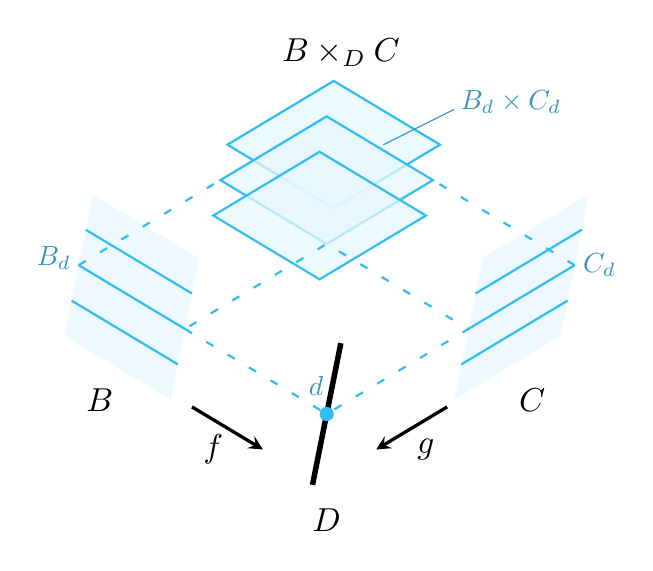
\begin{tikzpicture}[scale=.9]
        \draw [line width=2] (0, 0) -- (-.4, -2);
        \fill [cyan!7]
            (-2, 1.2) -- (-2.4, -.8) -- (-3.9, .1) -- (-3.5, 2.1);
        \fill [cyan!7]
            (2, 1.2) -- (1.6, -.8) -- (3.1, .1) -- (3.5, 2.1);
        \foreach \i in {1, ..., 3} {
            \draw [thick, cyan!80] 
                (-3.5 - .1 * \i, 2.1 - .5 * \i) -- (-2 - .1 * \i, 1.2 - .5 * \i)
                (3.5 - .1 * \i, 2.1 - .5 * \i) -- (2 - .1 * \i, 1.2 - .5 * \i);
        }
        \foreach \i in {1, ..., 3} {
            \draw [thick, cyan!80, fill=cyan!10, fill opacity=.75] 
                (-.1 * \i, 4.2 - .5 * \i) -- (1.5 - .1 * \i, 3.3 - .5 * \i) --
                (-.1 * \i, 2.4 - .5 * \i) -- (-1.5 - .1 * \i, 3.3 - .5 * \i) -- cycle;
        }
        \draw [thick, cyan!80, loosely dashed]
            (-2.2, .2) -- (-.2, -1) -- (1.8, .2) -- (-.2, 1.4) -- cycle
            (-3.7, 1.1) -- (-1.7, 2.3)
            (3.3, 1.1) -- (1.3, 2.3);
        \fill [cyan!80] (-.2, -1) circle (.1);
        \draw [line width=1.2, -stealth] (-2.1, -.9) -- (-1.1, -1.5);
        \draw [line width=1.2, -stealth] (1.5, -.9) -- (.5, -1.5);
        \node [cyan!75!black] at (-.35, -.6) {$d$};
        \node [scale=1.2] at (-.2, -2.5) {$D$};
        \node [scale=1.2] at (-3.4, -.8) {$B$};
        \node [scale=1.2] at (2.7, -.8) {$C$};
        \node [scale=1.2] at (-1.8, -1.5) {$f$};
        \node [scale=1.2] at (1.2, -1.5) {$g$};
        \node [scale=1.2] at (0, 4.1) {$B \times_D C$};
        \node [cyan!75!black] at (-4.05, 1.2) {$B_d$};
        \node [cyan!75!black] at (3.65, 1.1) {$C_d$};
        \node [cyan!75!black] at (2.4, 3.4) {$B_d \times C_d$};
        \draw [cyan!75!black] (1.6, 3.3) -- (.6, 2.8);
    \end{tikzpicture}\]
    $B \dtimes{D} C$ 被称为拉回, 也被称为是纤维积.
    \begin{definition} [拉回, 纤维积]
    \label{拉回}
    设 $\mathcal{C}$ 是 范畴 .
    对于 $\mathcal{C}$ 中的 交换图
    \[\begin{tikzcd}
	& B \\
	C & D
	\arrow["f"', from=1-2, to=2-2]
	\arrow["g", from=2-1, to=2-2]
    \end{tikzcd}\]
    如果这个图表具有 极限 ,
    就把这个极限叫做 $B, C$ 关于 $D$ 沿映射 $f, g$ 的\textbf{拉回}.

    具体地说, 该拉回是指交换图表
    \[\begin{tikzcd}
	{B \dtimes{D} C} & B \\
	C & D
	\arrow["{g'}", from=1-1, to=1-2]
	\arrow["{f'}"', from=1-1, to=2-1]
	\arrow["f"', from=1-2, to=2-2]
	\arrow["g", from=2-1, to=2-2]
    \end{tikzcd}\]
    它满足以下 万有性质 :
    对任意对象 $A' \in \mathcal{C}$, 如果有交换图表
    \[\begin{tikzcd}
	{A'} & B \\
	C & D
	\arrow["{g''}", from=1-1, to=1-2]
	\arrow["{f''}"', from=1-1, to=2-1]
	\arrow["f"', from=1-2, to=2-2]
	\arrow["g", from=2-1, to=2-2]
    \end{tikzcd}\]
    则存在唯一的态射 $h \colon A' \to A$, 使得以下图表交换:
    \[\begin{tikzcd}
	{A'} \\
	& {B \dtimes{D} C} & B \\
	& C & D
	\arrow["{\exists! h}"{description}, dashed, from=1-1, to=2-2]
	\arrow["{g''}", curve={height=-18pt}, from=1-1, to=2-3]
	\arrow["{f''}"', curve={height=18pt}, from=1-1, to=3-2]
	\arrow["{g'}"', from=2-2, to=2-3]
	\arrow["{f'}", from=2-2, to=3-2]
	\arrow["f"', from=2-3, to=3-3]
	\arrow["g", from=3-2, to=3-3]
    \end{tikzcd}\]
    \end{definition}
    而其对偶构造被称为推出, 也称为纤维余积, 比如说对于图表 
    \[\begin{tikzcd}
	& B \\
	C & D
	\arrow["f"', from=2-2, to=1-2]
	\arrow["g", from=2-2, to=2-1]
    \end{tikzcd}\]
    的推出记为 $B \dsqcup{D} C$. 它表示将两个对象沿着该态射粘接起来的过程.
\end{example}
\begin{exercise}
    请读者使用我们刚刚的思路思考拉回和推出分别代表什么, 此外, 说明拉回相当于``原像'', 推出相当于``像''.
\end{exercise}
接下来我们讲述极限的第二种刻画方式: 令 $I^{\triangleleft}$ 和 $I^{\triangleright}$ 为在 $I$ 中形式地添加一个始对象或终对象, 即将图表变为
\[\begin{tikzcd}
	& \varnothing \\
	i && j
	\arrow[from=1-2, to=2-1]
	\arrow[from=1-2, to=2-3]
	\arrow[from=2-1, to=2-3]
\end{tikzcd} \quad\text{和} \quad \begin{tikzcd}
	i && j \\
	& {*}
	\arrow[from=1-1, to=1-3]
	\arrow[from=1-1, to=2-2]
	\arrow[from=1-3, to=2-2]
\end{tikzcd}\]
此时有显然的函子 $I\to I^{\triangleleft}$ 和 $I \to I^{\triangleright}$. 此时考虑拉回(相当于限制态射对于 $\alpha$ 一点取逆)
\[\begin{tikzcd}
	{\Fct_\alpha{(I^{\triangleleft},\cal{C})}} & {\Fct(I^{\triangleleft},\cal{C})} \\
	{*} & {\Fct(I,\cal{C})}
	\arrow[from=1-1, to=1-2]
	\arrow[from=1-1, to=2-1]
	\arrow["{\text{限制}}"', from=1-2, to=2-2]
	\arrow["\alpha", from=2-1, to=2-2]
\end{tikzcd}\]
我们就得到 $\Fct_{\alpha}(I^{\triangleleft},\cal{C})$ 称其为锥, 此时其中对象可以表为(不难发现限制在 $I$ 上为 $\alpha$).
\[\begin{tikzcd}
	& X \\
	{\alpha(i)} && {\alpha(j)}
	\arrow[from=1-2, to=2-1]
	\arrow[from=1-2, to=2-3]
	\arrow["{\alpha(i\to j)}", from=2-1, to=2-3]
\end{tikzcd}\]
因此考虑其中终对象即为极限. 反过来, 考虑 $\Fct_{\alpha}(I^{\triangleright},\cal{C})$ 其始对象就是余极限.\\
现在, 我们在集合范畴 $\cate{Set}$ 中刻画极限, 这一过程相当于在求解规划问题\footnote{当然, 这样可能并不严谨.}
\begin{align*}
    \min & \quad \prolim \alpha \in \cal{C}\\
    \op{s.t.} &\left\{
    \begin{array}{ccc}
         \prolim \alpha \to \alpha(i),& \forall i\in \Obj(I) \\
         \alpha(i) \xrightarrow{\alpha(i\to j)} \alpha(j), & \forall (i\to j) \in \Mor(I)\\
         \text{上述全体箭头均交换}
    \end{array}
    \right.
\end{align*}
我们可以分成两步来求解该规划问题, 首先解决 $\prolim \alpha \to \alpha(i)$, 这无非是在说将 $I$ 先视为离散范畴进行求解, 直接得到结果为积 $\prod_{I} \alpha(i)$. 而后不断加入条件, 不难发现, 在集合范畴中, 增加这些条件相当于得到以下集合
\[
\left\{(x_i)_{i\in \Obj(I)} \colon \forall (i\xrightarrow{\sigma} j) \in\Hom(i,j), \alpha(\sigma)(x_i) = x_j\right\}.
\]
而该操作对于一般具体的范畴也是使用的, 这估计就是古老文献中, 将极限称为``普适问题的解''的原因所在.\\
现在我们来刻画余极限, 这与极限是对偶的.
\begin{align*}
    \max & \quad \indlim \alpha \in \cal{C}\\
    \op{s.t.} &\left\{
    \begin{array}{ccc}
           \alpha(i)\to \indlim \alpha,& \forall i\in \Obj(I) \\
         \alpha(i) \xrightarrow{\alpha(i\to j)} \alpha(j), & \forall (i\to j) \in \Mor(I)\\
         \text{上述全体箭头均交换}
    \end{array}
    \right.
\end{align*}
由于此时为 $\alpha(i) \to \indlim \alpha$, 因此我们可以先考虑 $\alpha(i) \xrightarrow{\alpha(i\to j)}\alpha(j)$, 这相当于说在生成元上具有一些关系 : 对于 $x_i \in \alpha(i)$, 有 $x_i \sim x_j \Leftrightarrow \alpha(i\to j)(x_i) = x_j$. \\
然后我们来考虑由此生成的 $\indlim \alpha$, 这无非是在说先使用 $\alpha(i)$ 自由生成 $\indlim \alpha$, 而后商去这些关系(读者可以想象为某种群展示, 当然群展示确实也是一种余极限), 得到:
\[
    \coprod_{i\in I} \alpha(i) /\sim
\]
但是目前我们只给出了关系, 我们想要具体刻画等价关系还需要再滤过范畴之上(或者说我们需要将 $\alpha(i)$ 和 $\alpha(j)$ 中的信息拉到某个具体的对象 $\alpha(k)$ 上, 由此更加精确地刻画等价关系), 首先容许我介绍一下何谓滤过:
\begin{definition}[滤过]
    非空范畴 $I$ 若满足以下条件, 则称是\textbf{滤过}的:
    \begin{itemize}
        \item 对于任意 $i,j \in \Obj(I)$, 存在 $k \in \Obj(I)$, 使得 $i \to k$, $j \to k$.
        \item 对于任意 $f,g \colon i \to j$ 存在 $k \in \Obj(I)$ 以及 $h \colon j \to k$ 使得 $hf = hg$.
    \end{itemize}
\end{definition}
此时前文生成的等价关系可以具体的写为
\[
   \text{存在}\left\{
   \begin{array}{cc}
       f\colon i \to k ,  \\
       g \colon j \to k 
   \end{array}\right.
   \quad \text{使得} \quad \alpha(f)(x_i) = \alpha(g)(x_j)\in \alpha(k)
\]
现在, 我们来给出一些日后经常打交道的例子.
\begin{example}[积, 余积, 等子, 余等子]
    \begin{enumerate}
        \item 如前文一般, 取 $I$ 为离散范畴, 不妨把 $I$ 等同于 $\Obj(I)$. 此时 $\indlim \alpha$ 称作对象 $X_i\coloneqq \alpha(i)$ 的\textbf{余积}, 写作 $\coprod_{i\in I} X_i$; 相应地, $\prod_{i\in I} X_i \coloneqq \prolim \alpha$ 称为对象 $X_i$ 的\textbf{积}.
        \item 取 $I = $
        \begin{tikzcd}
	\bullet & \bullet
	\arrow[shift left, from=1-1, to=1-2]
	\arrow[shift right, from=1-1, to=1-2]
        \end{tikzcd}
        给出的范畴(两个对象, 两个非 $\identity$ 的态射), 此时 $\alpha \colon I \to \cal{C}$ 可以描述为 
        \begin{tikzcd}
	X & Y
	\arrow["f", shift left, from=1-1, to=1-2]
	\arrow["g"', shift right, from=1-1, to=1-2]
        \end{tikzcd}
        我们想要探究这两个态射中``相同''的部分, 放在集合上看, 就是讨论 $f,g$ 在 $X$ 中上使得 $f(x) = g(x)$ 的部分, 但是我们现在的工作环境是范畴, 无法描绘对象内部的东西, 因此我们需要迂回一下(这目前看来可能并不严谨), 我们从外部视角来看``相同''的部分, 它满足的条件就是在说对于 $\phi \colon T \to X$, 若其``像''(记作 $\Image(\phi)$, 反映了 $\phi$ 在 $X$ 上的信息)落在``相同部分''(记作 $\ker(f,g)$) 之内, 则 $f\phi = g\phi$, 图解为我们总是有该图表交换
        \[\begin{tikzcd}
	&& T \\
	{\Image(\phi)} & {\ker(f,g)} & X & Y
	\arrow[from=1-3, to=2-1]
	\arrow["\phi", from=1-3, to=2-3]
	\arrow[from=1-3, to=2-4]
	\arrow[hook, from=2-1, to=2-2]
	\arrow[hook, from=2-2, to=2-3]
	\arrow["f", shift left, from=2-3, to=2-4]
	\arrow["g"', shift right, from=2-3, to=2-4]
        \end{tikzcd}\]
        因此, 我们需要取``最大''的那个($\Image \phi$)\footnote{当然,此处的``最大''指的是根据 $\hookrightarrow$ 的关系下最大的一个.}, 即 $\ker(f,g)$ 为 $\alpha$ 的极限 $\prolim \alpha$, 其泛性质相当于在说有以下图表交换
        \[\begin{tikzcd}
	& T \\
	{\ker(f,g)} & X & Y
	\arrow["{\exists !}"{description}, dashed, from=1-2, to=2-1]
	\arrow["\phi", from=1-2, to=2-2]
	\arrow[from=1-2, to=2-3]
	\arrow[hook, from=2-1, to=2-2]
	\arrow["f", shift left, from=2-2, to=2-3]
	\arrow["g"', shift right, from=2-2, to=2-3]
        \end{tikzcd}\]
        $\ker(f,g)$ 由于描述的是``相等''的部分, 因此不妨称其为\textbf{等子}.
        我们可以反过来, 问把 $f$ 和 $g$ 的信息粘起来, $Y$ 还剩下什么(记为 $\Coker(f,g)$). 这在集合中相当于说商集 $Y/\sim$, 其中 $\sim$ 为 $f(x) \sim g(x)$ 所生成的等价关系. 现在我们仍然从外部来刻画这一点, 这相当于说对于 $\psi \colon Y \to T$, 若 $\psi f = \psi g$ 那相当于说你不仅粘了, 可能还粘多了, 因此这个时候根据商的性质, 我们应当有 $\Coker(f,g) \to T$. 因此选出最大的对象(即始对象)作为 $\Coker(f,g)$, 即
        \[\begin{tikzcd}
	& T \\
	X & Y & {\Coker(f,g)}
	\arrow[from=2-1, to=1-2]
	\arrow["f", shift left, from=2-1, to=2-2]
	\arrow["g"', shift right, from=2-1, to=2-2]
	\arrow["\psi"', from=2-2, to=1-2]
	\arrow[from=2-2, to=2-3]
	\arrow[dashed, from=2-3, to=1-2]
        \end{tikzcd}\]
        根据先前的叙述, 相当于在说 $\Coker(f,g)$ 为 $\alpha$ 的余极限 $\indlim \alpha$.
        \item 现在我们可以更加正式的定义像和余像. 对于 $\cal{C}$ 中态射 $f \colon X \to Y$, 则像为 $f$ 在 $Y$ 中的信息全体, 考虑推出
        \[\begin{tikzcd}
	X & Y \\
	Y & {Y\dsqcup{X} Y}
	\arrow["f", from=1-1, to=1-2]
	\arrow["f"', from=1-1, to=2-1]
	\arrow[from=1-2, to=2-2]
	\arrow[from=2-1, to=2-2]
        \end{tikzcd}\]
        则 $Y \to Y\dsqcup{X}Y$ 相当于将 $f$ 带来的信息进行粘接, 因此可以将像定义为等子
        \[
        \Image (f) \coloneqq \ker \left( \begin{tikzcd}
	Y & {Y\dsqcup{X}Y}
	\arrow[shift left, from=1-1, to=1-2]
	\arrow[shift right, from=1-1, to=1-2]
        \end{tikzcd}\right)
        \]
        类似地, 我们可以讨论 $f$ 所反映的 $X$ 中的信息(在集合中, 将 $f(x) = f(y)$ 作为等价关系商去), 考虑拉回
        \[\begin{tikzcd}
	{X\dtimes{Y} X} & X \\
	X & Y
	\arrow[from=1-1, to=1-2]
	\arrow[from=1-1, to=2-1]
	\arrow["f"', from=1-2, to=2-2]
	\arrow["f", from=2-1, to=2-2]
        \end{tikzcd}\]
        则 $X\dtimes{Y} X \to X$ 相当于反映了 $f$ 中像相等的 $x$ 的等价类, 因此将余像定义为余等子
        \[
        \Coim(f) \coloneqq \Coker \left(
        \begin{tikzcd}
	{X\dtimes{Y} X} & X
	\arrow[shift left, from=1-1, to=1-2]
	\arrow[shift right, from=1-1, to=1-2]
        \end{tikzcd}
        \right)
        \]
        不难发现有典范态射
        \[\begin{tikzcd}
	X & Y \\
	{\Coim(f)} & {\Image(f)}
	\arrow["f", from=1-1, to=1-2]
	\arrow[two heads, from=1-1, to=2-1]
	\arrow[from=2-1, to=2-2]
	\arrow[hook, from=2-2, to=1-2]
        \end{tikzcd}\]
        读者可以验证: 
        \begin{center}
            $f$ 满 $\Leftrightarrow$ $\Image(f) \rightiso Y$ 且 $f$ 单 $\Leftrightarrow$ $X\rightiso \Coim(f)$
        \end{center}
        但是 $\Coim(f)$ 不一定同构于 $\Image(f)$, 因此即单又满的态射不一定是同构. 当 $\Coim(f) \rightiso \Image(f)$ 时, 我们称 $f$ 为\textbf{严格}态射.
    \end{enumerate}
\end{example}
注意到, 在一般的范畴 $\cal{C}$ 中, 函子 $\alpha$ 的极限或余极限不总是存在, 我们比较喜欢在对于任意小范畴 $I$, (余)极限总是存在的范畴上工作, 这种性质我们称为完备性(当然, 你完全可以类比为我们在完备的度量空间中工作, 这是没有任何问题的.)
\begin{definition}[完备]
    对于范畴 $\cal{C}$, 若对所有小范畴 $I$, 所有以 $I$ 为指标的 $\indlim$ 都存在, 则称之为\textbf{完备}的, 若所有以 $I$ 为指标的 $\prolim$ 都存在, 则称之为\textbf{余完备}的.
\end{definition}
\begin{example}
    \begin{itemize}
        \item 根据我们前文在 $\cate{Set}$ 上的构造可知 $\cate{Set}$ 是完备且余完备的.
        \item 在拓扑空间中, 我们有极限拓扑和余极限拓扑, 它搭配上对应的极限与余极限集合即可得到极限与余极限拓扑空间.
        \item 群范畴 $\cate{Grp}$ 也是完备的, 极限和余极限的构造与集合是一致的. 在群范畴中, 推出即为融合积.
    \end{itemize}
\end{example}

\subsection{应用 : Kan 延拓}
现在, 我们考虑范畴 $\cal{C},D,E$, 以及函子 $\mathcal{C} \xrightarrow{K}\cal{D}$ , $\mathcal{C} \xrightarrow{F} \mathcal{E}$, 如图所示
\[\begin{tikzcd}
	{\mathcal{C}} \\
	{\mathcal{D}} & {\mathcal{E}}
	\arrow["K"', from=1-1, to=2-1]
	\arrow["F", curve={height=-12pt}, from=1-1, to=2-2]
	\arrow["{?}"{description}, dashed, from=2-1, to=2-2]
\end{tikzcd}\]
我们希望找到函子 $L\colon \mathcal{D} \to \mathcal{E}$ 使得 $LK$ 逼近于 $F$. 和极限一般, 我们有两种逼近方式, 一种是从较大的一侧往小逼近, 一种是较小一侧往大逼近.\\

不妨将``较大''的 $LK$ 放在左手, 较小的 $LK$ 放在右手, 回忆我们在第~\ref{函子范畴}~节对于函子与自然变换的看法, 可以得到
\[\begin{tikzpicture}[x=0.75pt,y=0.75pt,yscale=-1,xscale=1]
%uncomment if require: \path (0,300); %set diagram left start at 0, and has height of 300

%Straight Lines [id:da7102542369090952] 
\draw    (393.11,124.17) -- (414.11,124.17) ;
\draw [shift={(416.11,124.17)}, rotate = 180] [color={rgb, 255:red, 0; green, 0; blue, 0 }  ][line width=0.75]    (10.93,-3.29) .. controls (6.95,-1.4) and (3.31,-0.3) .. (0,0) .. controls (3.31,0.3) and (6.95,1.4) .. (10.93,3.29)   ;
%Straight Lines [id:da7341960176956119] 
\draw    (457.11,124.17) -- (478.11,124.17) ;
\draw [shift={(480.11,124.17)}, rotate = 180] [color={rgb, 255:red, 0; green, 0; blue, 0 }  ][line width=0.75]    (10.93,-3.29) .. controls (6.95,-1.4) and (3.31,-0.3) .. (0,0) .. controls (3.31,0.3) and (6.95,1.4) .. (10.93,3.29)   ;
%Straight Lines [id:da6127211899518781] 
\draw    (525.11,123.17) -- (546.11,123.17) ;
\draw [shift={(548.11,123.17)}, rotate = 180] [color={rgb, 255:red, 0; green, 0; blue, 0 }  ][line width=0.75]    (10.93,-3.29) .. controls (6.95,-1.4) and (3.31,-0.3) .. (0,0) .. controls (3.31,0.3) and (6.95,1.4) .. (10.93,3.29)   ;
%Straight Lines [id:da9966989226172298] 
\draw    (346.11,125.17) -- (363.11,125.17) ;
\draw [shift={(365.11,125.17)}, rotate = 180] [color={rgb, 255:red, 0; green, 0; blue, 0 }  ][line width=0.75]    (10.93,-3.29) .. controls (6.95,-1.4) and (3.31,-0.3) .. (0,0) .. controls (3.31,0.3) and (6.95,1.4) .. (10.93,3.29)   ;
%Straight Lines [id:da9273012188666165] 
\draw    (89.11,125.17) -- (106.11,125.17) ;
\draw [shift={(108.11,125.17)}, rotate = 180] [color={rgb, 255:red, 0; green, 0; blue, 0 }  ][line width=0.75]    (10.93,-3.29) .. controls (6.95,-1.4) and (3.31,-0.3) .. (0,0) .. controls (3.31,0.3) and (6.95,1.4) .. (10.93,3.29)   ;
%Straight Lines [id:da24458156378074092] 
\draw    (149.11,125.17) -- (166.11,125.17) ;
\draw [shift={(168.11,125.17)}, rotate = 180] [color={rgb, 255:red, 0; green, 0; blue, 0 }  ][line width=0.75]    (10.93,-3.29) .. controls (6.95,-1.4) and (3.31,-0.3) .. (0,0) .. controls (3.31,0.3) and (6.95,1.4) .. (10.93,3.29)   ;
%Straight Lines [id:da039540146815657096] 
\draw    (218.11,125.17) -- (235.11,125.17) ;
\draw [shift={(237.11,125.17)}, rotate = 180] [color={rgb, 255:red, 0; green, 0; blue, 0 }  ][line width=0.75]    (10.93,-3.29) .. controls (6.95,-1.4) and (3.31,-0.3) .. (0,0) .. controls (3.31,0.3) and (6.95,1.4) .. (10.93,3.29)   ;
%Straight Lines [id:da2812032899568666] 
\draw    (287.11,125.17) -- (304.11,125.17) ;
\draw [shift={(306.11,125.17)}, rotate = 180] [color={rgb, 255:red, 0; green, 0; blue, 0 }  ][line width=0.75]    (10.93,-3.29) .. controls (6.95,-1.4) and (3.31,-0.3) .. (0,0) .. controls (3.31,0.3) and (6.95,1.4) .. (10.93,3.29)   ;
%Straight Lines [id:da7961883799165974] 
\draw  [dash pattern={on 0.84pt off 2.51pt}]  (70.11,165.5) -- (304.11,165.5)(70.11,168.5) -- (304.11,168.5) ;
\draw [shift={(312.11,167)}, rotate = 180] [color={rgb, 255:red, 0; green, 0; blue, 0 }  ][line width=0.75]    (10.93,-3.29) .. controls (6.95,-1.4) and (3.31,-0.3) .. (0,0) .. controls (3.31,0.3) and (6.95,1.4) .. (10.93,3.29)   ;
%Straight Lines [id:da543630385168764] 
\draw  [dash pattern={on 0.84pt off 2.51pt}]  (591,168.5) -- (362.11,168.5)(591,165.5) -- (362.11,165.5) ;
\draw [shift={(354.11,167)}, rotate = 360] [color={rgb, 255:red, 0; green, 0; blue, 0 }  ][line width=0.75]    (10.93,-3.29) .. controls (6.95,-1.4) and (3.31,-0.3) .. (0,0) .. controls (3.31,0.3) and (6.95,1.4) .. (10.93,3.29)   ;
%Shape: Lamp [id:dp27791867232559975] 
\draw  [fill={rgb, 255:red, 248; green, 231; blue, 28 }  ,fill opacity=1 ] (321,173.97) -- (321,161.51) .. controls (321,158.38) and (324.39,155.84) .. (328.56,155.84) .. controls (332.73,155.84) and (336.11,158.38) .. (336.11,161.51) -- (336.11,173.97) -- (321,173.97) -- cycle (324.02,178.51) -- (324.02,167.17) .. controls (324.02,165.3) and (326.05,163.77) .. (328.56,163.77) .. controls (331.06,163.77) and (333.09,165.3) .. (333.09,167.17) -- (333.09,178.51) ;
%Straight Lines [id:da2531485777379041] 
\draw [color={rgb, 255:red, 155; green, 155; blue, 155 }  ,draw opacity=0.5 ][line width=3]    (591,168.5) -- (374,168.5)(591,165.5) -- (374,165.5) ;
%Shape: Free Drawing [id:dp0409551019615928] 
\draw  [color={rgb, 255:red, 0; green, 0; blue, 0 }  ,draw opacity=1 ][line width=5.25] [line join = round][line cap = round] (374.22,166.67) .. controls (374.22,166.67) and (374.22,166.67) .. (374.22,166.67) ;

% Text Node
\draw (321,118.4) node [anchor=north west][inner sep=0.75pt]    {$F$};
% Text Node
\draw (364,117.4) node [anchor=north west][inner sep=0.75pt]    {$L_{1} K$};
% Text Node
\draw (416,116.4) node [anchor=north west][inner sep=0.75pt]    {$L_{2} K$};
% Text Node
\draw (483,116.4) node [anchor=north west][inner sep=0.75pt]    {$L_{3} K$};
% Text Node
\draw (558,117.4) node [anchor=north west][inner sep=0.75pt]    {$\cdots $};
% Text Node
\draw (243,117.4) node [anchor=north west][inner sep=0.75pt]    {$L_{1} 'K$};
% Text Node
\draw (350,176) node [anchor=north west][inner sep=0.75pt]   [align=left] {接近 $\displaystyle F$};
% Text Node
\draw (269,176) node [anchor=north west][inner sep=0.75pt]   [align=left] {接近$\displaystyle F$};
% Text Node
\draw (171,117.4) node [anchor=north west][inner sep=0.75pt]    {$L_{2} 'K$};
% Text Node
\draw (112,117.4) node [anchor=north west][inner sep=0.75pt]    {$L_{3} 'K$};
% Text Node
\draw (55,176) node [anchor=north west][inner sep=0.75pt]   [align=left] {远离 $\displaystyle F$};
% Text Node
\draw (552,176) node [anchor=north west][inner sep=0.75pt]   [align=left] {远离 $\displaystyle F$};
% Text Node
\draw (58,118.4) node [anchor=north west][inner sep=0.75pt]    {$\cdots $};


\end{tikzpicture}\]
其中箭头均为自然变换, 现在我们寻求对于 $F$ 的逼近, 就相当于说以 $F$ 为中心, 我们向从某一侧往中间逼近(即为图中带虚线的箭头).\\
现在我们以从右向左的逼近为例, 此时不妨将 $F$ 视为灯泡(图中亮黄灯的), 而取定的函子 $L$ 为一个物体, 则灯泡产生的影子即为 $L$ 可以往``更小''的对象中投射自然变换的部分. 因此最接近于 $F$ 的 $LK$ 应当对于任意``小于'' $F$ 的 $L';K$ 的$L'$ 都带有自然变换 $L \Rightarrow L'$. 我们将如此得到的 $L$ 称为 $F$ 沿着 $K$ 的左 Kan 延拓, 对偶地, 从左侧往右的逼近称为右 Kan 延拓.
\begin{definition}[Kan延拓]\label{Def:Kan延拓}
    考虑范畴$\mathcal{C,D,E}$间的图表
    \[\begin{tikzcd}
	{\mathcal{C}} \\
	{\mathcal{D}} & {\mathcal{E}}
	\arrow["K"', from=1-1, to=2-1]
	\arrow["F", curve={height=-10pt}, from=1-1, to=2-2]
    \end{tikzcd}\]
    其中$K \colon \mathcal{C} \to \mathcal{D}$, $F\colon \mathcal{C} \to \mathcal{E}$.
    \begin{itemize}
        \item 函子$F$沿$K$的左Kan延拓意谓以下资料$(\Lan_K F,\eta)$,其中
        \begin{itemize}
            \item $\Lan_KF\colon \mathcal{D} \to \mathcal{E}$是函子.
            \item $\eta \colon F\to (\Lan_K F)K$是函子间的态射.
        \end{itemize}
        使得以下泛性质成立:对任何资料$L \colon\mathcal{D} \to \mathcal{E}$,和$\xi \colon F \to LK$,存在唯一的态射$\chi\colon \Lan_K F \to L$使得$\xi = (\chi K)\eta$(态射的纵横合成),或以2-胞腔图解为
        \[\begin{tikzcd}
	{\mathcal{C}} \\
	{\mathcal{D}} & {\mathcal{E}}
	\arrow["K"', from=1-1, to=2-1]
	\arrow[""{name=0, anchor=center, inner sep=0}, "F", curve={height=-12pt}, from=1-1, to=2-2]
	\arrow["L"', from=2-1, to=2-2]
	\arrow["\xi"{description}, shorten <=4pt, Rightarrow, from=0, to=2-1]
        \end{tikzcd}=
        \begin{tikzcd}
	{\mathcal{C}} \\
	{\mathcal{D}} & {\mathcal{E}}
	\arrow["K"', from=1-1, to=2-1]
	\arrow[""{name=0, anchor=center, inner sep=0}, "F", curve={height=-12pt}, from=1-1, to=2-2]
	\arrow[""{name=1, anchor=center, inner sep=0}, "{\Lan_K F}"', from=2-1, to=2-2]
	\arrow[""{name=2, anchor=center, inner sep=0}, "L"', curve={height=30pt}, from=2-1, to=2-2]
	\arrow["\eta"{description}, shorten <=4pt, Rightarrow, from=0, to=2-1]
	\arrow["\chi", shorten <=7pt, shorten >=2pt, Rightarrow, from=1, to=2]
    \end{tikzcd}\]
    \item 函子$F$沿$K$的右延拓意谓以下资料$(\Ran_K F , \varepsilon)$,其中
    \begin{itemize}
        \item $\Ran_K F\colon \mathcal{D} \to \mathcal{E}$是函子.
        \item $\varepsilon\colon (\Ran_K F)K \to F$是函子间的态射.
    \end{itemize}
    使得以下泛性质成立:对任何资料$R \colon \mathcal{D} \to \mathcal{E}$和$\delta \colon RK \to F$,存在唯一的$\theta \colon R \to (\Ran_KF)K$使得$\delta = \varepsilon(\theta K)$,或用2-胞腔图解为
    \[\begin{tikzcd}
	{\mathcal{C}} \\
	{\mathcal{D}} & {\mathcal{E}}
	\arrow["K"', from=1-1, to=2-1]
	\arrow[""{name=0, anchor=center, inner sep=0}, "F", curve={height=-12pt}, from=1-1, to=2-2]
	\arrow["R"', from=2-1, to=2-2]
	\arrow["\delta"{description}, shorten >=4pt, Rightarrow, from=2-1, to=0]
\end{tikzcd}=\begin{tikzcd}
	{\mathcal{C}} \\
	{\mathcal{D}} & {\mathcal{E}}
	\arrow["K"', from=1-1, to=2-1]
	\arrow[""{name=0, anchor=center, inner sep=0}, "F", curve={height=-12pt}, from=1-1, to=2-2]
	\arrow[""{name=1, anchor=center, inner sep=0}, "{\Ran_K F}"', from=2-1, to=2-2]
	\arrow[""{name=2, anchor=center, inner sep=0}, "R"', curve={height=30pt}, from=2-1, to=2-2]
	\arrow["\varepsilon"{description}, shorten >=4pt, Rightarrow, from=2-1, to=0]
	\arrow["\theta", shorten <=2pt, shorten >=7pt, Rightarrow, from=2, to=1]
    \end{tikzcd}\]
    \end{itemize}
\end{definition}
使用函子范畴 $\mathcal{E}^{\mathcal{C}}$ 以及 $\mathcal{E}^{\mathcal{D}}$ 的概念, 可以发现左, 右 Kan 延拓分别在说有双射
\begin{align*}
    \Hom_{\mathcal{E}^{\mathcal{D}}}(\Lan_K F,L) &\xrightarrow{1:1} \Hom_{\mathcal{E}^{\mathcal{C}}}(F,LK)\\
    \chi &\mapsto (\chi K)\eta,\\
    \Hom_{\mathcal{E}^{\mathcal{D}}}(R,\Ran_K F) &\xrightarrow{1:1} \Hom_{\mathcal{E}^{\mathcal{C}}}(RK,F)\\
    \theta &\mapsto \varepsilon(\theta K);
\end{align*}
证明这一点只需要观察到 $\xi \colon F \Rightarrow L$ 都唯一确定了一个 $\chi$, 而 $\chi$ 又可以反向决定 $\xi = (\chi K)\eta$ 即可. \\
此外 Kan 延拓还有诸多的性质, 不过受限于本文讲解顺序, 将会在伴随函子之后讲解.
\subsection{可表函子,自由余完备化}
本节将介绍一些``广义对象'', 可以理解为漂浮在范畴上的幽灵, 事实上, 一般的函子都可以视为这样的广义对象, 不过目前我们主要关注取值在集合上的情况, 这种广义对象称为(集合)预层, 该定义有一些拓扑学渊源, 我们先来看拓扑空间上的情况.
\begin{definition}[$\mathcal{D}$-值预层]
    令 $X$ 为拓扑空间, $\mathcal{D}$为范畴, $\open(X)$为$X$上开集构成(以包含关系作为态射)的范畴.则$X$上的$\mathcal{D}$-值预层$\mathcal{F}$就是一个函子
    \[
        \mathcal{F}: \open(X)^{\opposite} \to \mathcal{D}
    \]
    也即$\open(X)$到$\mathcal{D}$的一个反变函子.将全体$\mathcal{D}$-值预层构成的范畴记为$\presheaves(\open(X),\mathcal{D})$,特别地,取$\mathcal{D} = \operatorname{Set}$时记为$\open(X)^{\land}$.
\end{definition}
这样的定义有些许的抽象,但是我们可以将其显式的写出来\footnote{抄的预层的代码.}
\begin{definition}
    设 $X$ 是拓扑空间, $\mathcal{D}$ 是范畴.
    则 $X$ 上取值于 $\mathcal{D}$ 的\textbf{预层} $\mathcal{F}$
    由以下信息组成:
    \begin{itemize}
        \item
            对每个开集 $U \subset X$, 有一个对象
            \[
                \mathcal{F} (U) \in \mathcal{D},
            \]
            称为 $U$ 上 $\mathcal{F}$ 的所有\textbf{截面}构成的空间.
        \item
            对任两个开集 $U \subset V \subset X$, 有一个 $\mathcal{D}$ 中的态射
            \[
                \operatorname{res}_U^V
                \colon \mathcal{F} (V) \to \mathcal{F} (U),
            \]
            称为\textbf{限制映射}.
            这个映射通常也记为 $(-)|_U$.

            限制映射还满足如下函子性要求:
            \begin{itemize}
                \item $\operatorname{res}_U^U = \identity_{\mathcal{F} (U)}$.
                \item 对于任意满足 $U \subset V \subset W$ 的开集,都有 
                $\operatorname{res}_U^W = \operatorname{res}_U^V \circ 
                \operatorname{res}_V^W$.
            \end{itemize}
    \end{itemize}
    当 $\mathcal{D} = \mathsf{Set}$ 为集合范畴时,
    通常称 $\mathcal{F}$ 为\textbf{集合预层};
    当 $\mathcal{D} = \mathsf{Ab}$ 为Abel 群范畴时,
    通常称 $\mathcal{F}$ 为\textbf{Abel 预层}, 以此类推.
\end{definition}
\begin{remark}
    不妨将预层视为 $U$ 上一堆函数的集合, 而限制映射此时就可以视为函数的限制, 因此自然为反变函子.
\end{remark}
接下来将定义推广到一般范畴上, 不难发现 $\presheaves(\mathcal{C},\mathcal{D})$ 即为 $\Fct(\mathcal{C}^{\opposite},\mathcal{D})$. 本节取 $\mathcal{D} = \cate{Set}$, 将对应预层范畴记为 $\mathcal{C}^{\wedge}$.\\
此外, 还可以定义 
\[
    \mathcal{C}^{\vee} \coloneqq \Fct(\mathcal{C}^{\opposite},\cate{Set}^{\opposite}) = \Fct(\mathcal{C},\cate{Set})^{\opposite}.
\]
接下来观察 $\Hom$-集, 不难发现 $\Hom$-集实际上可以视为双函子 
\begin{align*}
    \Hom \colon \mathcal{C}^{\opposite} \times \mathcal{C} &\to \cate{Set}\\
    (X,Y) &\mapsto \Hom_{\cal{C}}(X,Y).
\end{align*}
前一个 $\mathcal{C}$ 为反变的原因在于 $f \colon X' \to X$ 可以诱导拉回 $(X \xrightarrow{a} Y) \mapsto (X' \xrightarrow{a\circ f}Y) \in \Hom(X',Y)$.\\
现在, 我们只选定一个部分, 得到函子 $h_{\mathcal{C}}$ 与 $k_{\mathcal{C}}$ 如下
\begin{align*}
    h_{\mathcal{C}} \colon \mathcal{C} &\to \mathcal{C}^{\wedge}\\
    S &\mapsto \Hom_{\cal{C}}(-,S)\\
    k_{\mathcal{C}} \colon \mathcal{C} &\to \mathcal{C}^{\vee}\\
    S &\mapsto \Hom(S,-).
\end{align*}
此时具有自然地求值函子
\[
\ev^{\wedge} \colon \mathcal{C}^{\opposite}\times \mathcal{C}^{\wedge} \to \cate{Set}, \quad (S,A) \mapsto A(S)
\]
以及对偶版本. 
我们有以下重要引理
\begin{theorem}[Yoneda]
    对于 $S \in \Obj(\mathcal{C})$ 以及 $A \in \Obj(\mathcal{C}^{\land})$ 映射
    \begin{align*}
        \Hom_{\mathcal{C}^{\wedge}}(h_{\mathcal{C}}(S),A) &\to A(S)\\
        \left(\Hom_{\cal{C}}(-,S)\xRightarrow{\phi} A(-)\right) &\mapsto \phi_S(\identity_S)
    \end{align*}
    为双射; 它给出函子的同构 $\Hom_{\cal{C}^{\wedge}}(h_{\mathcal{C}}(-),-) \rightiso \ev^{\wedge}$. 函子 $h_{\cal{C}}$ 是全忠实的.\\
    反之可以得到对偶情况.
\end{theorem}
\begin{proof}
    该证明其实是无趣的集合论证明, 只需证明上述映射可逆. 也就是说对于 $A(S)$ 中的元素 $u_S$, 我们要将其视为某个自然变换 $\phi$ 的像 $\phi_S(\identity_S)$, 而后反向构造出对应的 $\phi$ 即可. 考虑图表
    \[\begin{tikzcd}
	{\identity_S} & {\Hom_{\cal{C}}(S,S)} & {A(S)} & {u_S} \\
	f & {\Hom_{\cal{C}}(T,S)} & {A(T)} & { A(f)(u_S)}
	\arrow["\in"{marking, allow upside down}, draw=none, from=1-1, to=1-2]
	\arrow[maps to, from=1-1, to=2-1]
	\arrow["{\phi_S}", from=1-2, to=1-3]
	\arrow["{f^{}*}"', from=1-2, to=2-2]
	\arrow["{A(f)}", from=1-3, to=2-3]
	\arrow["\in"{marking, allow upside down}, draw=none, from=1-4, to=1-3]
	\arrow[maps to, from=1-4, to=2-4]
	\arrow["\in"{marking, allow upside down}, draw=none, from=2-1, to=2-2]
	\arrow["{\phi_T}"', from=2-2, to=2-3]
	\arrow["\in"{marking, allow upside down}, draw=none, from=2-4, to=2-3]
    \end{tikzcd}\]
    道尽半切. 此时显然有 $\phi_S(\identity_S) = u_S$, 而根据图表交换性可知 $A(f)\phi_S(\identity_S) = \phi_T(f)$, 由此又给出 $\phi\colon \Hom_{\mathcal{C}}(-,S) \xRightarrow{\phi} A(-)$.\\
    至于全忠实性考虑 $A = h_{\mathcal{C}}(T)$, 得到 
    \[
    \Hom_{\mathcal{C}^{\wedge}}(h_{\mathcal{C}}(S),h_{\mathcal{C}}(T)) \rightiso \Hom_{\mathcal{C}}(T,S).
    \]
\end{proof}
\begin{remark}
    Yoneda 引理告诉我们,
范畴中的对象由所有别的对象到它的态射所完全描述.
例如, 对一个拓扑空间 $X$ 而言,
如果对任何别的拓扑空间 $Y$,
都知道从 $Y$ 到 $X$ 的所有连续映射构成的集合 $\Hom_{\mathsf{Top}} (Y, X)$ 是什么样,
那我们也就能知道 $X$ 是哪个拓扑空间.
换言之, 我们可以用别的空间 $Y$ 来 ``探测'' $X$ 的拓扑.\\
Yoneda 观点是指, 对于范畴中的对象 $X$ 而言,
我们将 $X$ 等同于别的对象到它的态射的信息, 我们暂且成为 ``探测信息''.
这样, 一份合理的探测信息应该(通过同构)能确定(预层)范畴中的对象.
然而, 有时这样的对象实际并不在原来的范畴中, 我们就称其被该对象被该信息表出.
\end{remark}
\begin{definition}[可表性]
    称 $A \colon \mathcal{C}^{\opposite} \to \cate{Set}$ 是可表函子, 如果存在 $X \in \Obj(\cal{C})$ 以及同构 $\phi \colon h_{\cal{C}}(X) \rightiso A$. 此时称 $(X,\phi)$ 表出了 $A$, 称其为代表元.
\end{definition}
\begin{remark}
    由 Yoneda 引理的证明可知: 给定资料 $(X,\phi)$ 相当于给定 $(X,u)$ 其中 $u = \phi_X(\identity_X) \in A(X)$.
\end{remark}
有鉴于此, 可以使用 $(X,u)$, $u\in A(X)$ 来表述 $A$, 此时称 $u$ 为泛族; 这起源于模空间的研究.
\begin{lemma}
    若 $A$ 可被 $(X,\phi)$ 所表出, 则代表元在相差至多一个同构的意义下是唯一的.
\end{lemma}
\begin{proof}
    留作习题.
\end{proof}
\begin{example}[子对象分类子]
    在 $\cate{Set}$ 中, 任意子集 $A \subset X$ 都对应于特征映射 $\chi_A\colon X \to \{0,1\}$, 将 $A$ 中元素对应于 $1$ 而其它元素为 $0$. 使得我们有拉回图表
    \[\begin{tikzcd}
	A & {\{1\}} \\
	X & {\{0,1\}}
	\arrow[from=1-1, to=1-2]
	\arrow[hook, from=1-1, to=2-1]
	\arrow["{\text{子对象分类子}}", hook, from=1-2, to=2-2]
	\arrow["{\chi_A}"', from=2-1, to=2-2]
    \end{tikzcd}\]
    可以视为对于 $X$ 的``分类''. \\
    在范畴 $\cal{C}$ 中, 若存在拉回且子对象函子(定义~\ref{定义-子对象}) $\Sub \colon \cal{C}^{\opposite} \to \cate{Set}$ 可表, 则存在 $\Omega$ 使得
    \[
    \Sub_{\cal{C}}(X) \simeq \Hom_{\cal{C}}(X,\Omega)
    \]
    此时 $\Omega$ 称为 $\cal{C}$ 的子对象分类子.\\
    由前文不难看出 $\{0,1\}$ 为 $\cate{Set}$ 的子对象分类子.因此我们可以得知 $\Hom_{\cate{Set}}(X,\{0,1\}) = \Sub_{\cal{C}}(X) = \mathcal{P}(X)$. 即幂集可表. \footnote{这也是某群入群题的fancy解法.}
\end{example}
\begin{example}[Eilenberg-Maclane 空间]
    Eilenberg-Maclane 空间 $X = K(M,n)$ 为使得 $\pi_n(X) \simeq M$ 而 对于 $k \neq n$ 有 $\pi_k(X) =0 $ 的 CW 复形. 它表示了约化上同调函子 $H^n(-,M)$, 即 
    \[
    H^n(-;M) \simeq [-,K(M,n)]_* = \Hom_{h\cate{Top}_*}(-,K(M,n)).
    \].
    在\cite{aguilar2002algebraic}中, 就使用上述定义直接定义出上同调.
\end{example}
\subsubsection{题外话:上同调理论与 Brown 可表定理}
\begin{remark}
    本节为题外话, 乖宝宝不要看. $[X,Y]_* = \Hom_{h\cate{An}_*}(X,Y)$
\end{remark}
令 $\cate{An}$ 为空间(Kan 复形)构成的 $\infty$-范畴\footnote{或称生象范畴, 但是由于我们考虑带点空间, 因此使用空间一词.}, 则
\begin{definition}
    二元组 $(E^*,\partial)$ 被称为是上同调理论, 指
    \[
    E^* \colon h\cate{An}_* \to \cate{grAb}
    \]
    为从带点空间范畴的同伦范畴到分次 Abel 群范畴的函子, 且
    \[
    \partial \colon E^* \simeq E^{*+1}\circ \Sigma
    \]
    为自然同构, 满足以下条件
    \begin{enumerate}
        \item 对于每族带点空间 $\{X_{\alpha}\}_{\alpha \in A}$ 自然映射
        \[
        E^*(\coprod_{\alpha \in A}X_{\alpha}) \to \prod_{\alpha \in A}E^*(X_{\alpha})
        \]
        为同构. 特别地 $E^*(*) \simeq 0$.
        \item 对于余纤维列
        \[
        X' \to X \to X''
        \]
        有正合列
        \[
        E^*(X'') \to E^*(X) \to E^*(X').
        \]
    \end{enumerate}
\end{definition}
\begin{example}
    对于带点空间 $X$, 其约化上同调 $\tilde{H}^*(X)$ 为上同调理论.
\end{example}
此时, 我们有如下的表示定理
\begin{theorem}[Brown 可表定理]\label{定理-Brown 可表}
    令 $h\cate{An}_*^{\geq 0}$ 为连通带点空间范畴的同伦范畴. 则函子 $F \colon (h\cate{An}_*^{\geq 0})^{\opposite}\to \cate{Set}$ 可表当且仅当其具有以下两个性质:
    \begin{enumerate}
        \item 对于每族连通带点空间 $\{X_{\alpha}\}_{\alpha \in A}$, 有双射
        \[
        F(\bigvee_{\alpha \in A}X_{\alpha}) \to \prod_{\alpha \in A}F(X_{\alpha})
        \]
        \item 对于每个 $\cate{An}_*^{\geq 0}$ 中的推出图表
        \[\begin{tikzcd}
	X & Y \\
	{X'} & {Y'}
	\arrow[from=1-1, to=1-2]
	\arrow[from=1-1, to=2-1]
	\arrow[from=1-2, to=2-2]
	\arrow[from=2-1, to=2-2]
        \end{tikzcd}\]
        有满射
        \[
        F(Y') \to F(X') \dtimes{F(X)} F(Y)
        \]
    \end{enumerate}
\end{theorem}
\begin{proof}
    将在第~\ref{稳定同伦一瞥}~中证明.
\end{proof}
\begin{corollary}
    令 $E \colon h\cate{An}_* \to \cate{grAb}$ 为上同调理论. 则存在唯一的一族带点空间 $E_n \in \cate{An}_*$ 以及同伦等价
    \[
    \delta_n \colon E_n \xrightarrow{\Omega}E_{n+1}
    \]
    使得有自然同构
    \[
    \varphi_n \colon E^n(X) \simeq [X,E_n]_*
    \]
    且 $\partial \colon E^n(X) \simeq E^{n+1}(\Sigma X)$ 由下式给出
    \[
    E^n(X) \simeq [X,E_n]_* \simeq [X,\Omega E_{n+1}]_* \simeq [\Sigma X, E_{n+1}]_* \simeq E^{n+1}(\Sigma X).
    \]
\end{corollary}
\begin{proof}
    同上.
\end{proof}
这告诉我们可以定义出以下一列空间
\begin{definition}[拓扑谱]
    \textbf{拓扑谱} $E = (\{E_n\}_{n\in \Z}, \delta_n)$ 由以下信息构成:
    \begin{itemize}
        \item 一列带点空间 $X_0,X_1, \cdots$
        \item 对任何 $n \geq 0$, 有带点映射 $\sigma_n \colon \Sigma X_n \to X_{n+1}$.
    \end{itemize}
    称 $X$ 为 \textbf{$\Omega$-谱}, 若:
    \begin{itemize}
        \item 对任何 $n \geq 0$ 有 $\sigma_n$ 诱导的 $X_n \to \Omega X_{n+1}$ 为弱同伦等价.
    \end{itemize}
    准确来说, 可以定义 $\Omega$-谱的 $\infty$-范畴为
    \[
    \cate{Sp} \simeq \prolim \left(\cate{An}_* \xleftarrow{\Omega} \cate{An}_* \xleftarrow{\Omega}\cate{An}_* \xleftarrow{\Omega} \cdots\right)
    \]
\end{definition}
对于经典的上同调理论 $\tilde{H}^*(-,M)$ 使用定理~\ref{定理-Brown 可表}可以给出谱 $HM$, 称为 \textbf{Eilenberg-Maclane 谱}, 此时
\[
\pi_n(HM_m) = [S^n , HM_m]_* = \tilde{H}^n(S^n,M) = \left\{
\begin{array}{cc}
     M,& n=m \\
     0,& \text{其它} 
\end{array}\right.
\]
因此此时 $HM_m$ 实际为 Eilberg-Maclane 空间 $K(M,n)$.
\subsection{伴随函子}
(未完待续)
\subsection{幺半范畴}
\subsection{群对象}
\section{方便的空间范畴}
本节来讲述方便的空间范畴概念, 一般来说, 方便的空间范畴指的是拓扑空间范畴中满足以下条件的饱和\footnote{replete, 子范畴 $\cal{D}$ 称为是饱和的, 指对于任意 $x\in \cal{D}$, 若在 $\cal{C}$ 中有 $f \colon y \simeq x$, 则 $f$ 和 $y$ 都在 $\cal{D}$ 中.}全子范畴. 本节主要参考\cite{StricklandCGWH}以及\cite[7.好用的空间范畴]{李思}
\begin{definition}[方便的空间范畴]
    称 $\cal{C}$ 为\textbf{方便的空间范畴}, 指其为 $\cate{Top}$ 的饱和全子范畴, 并且满足以下三条条件
    \begin{itemize}
        \item 每个 CW 复形均为 $\cal{C}$ 中的对象.
        \item $\cal{C}$ 是 Cartesian 闭的(定义~\ref{定义:Cartesian闭}, 或者说具有指数律).
        \item $\cal{C}$ 是完备且余完备的.
    \end{itemize}
\end{definition}
首先介绍闭幺半范畴的概念
\begin{definition}[闭幺半范畴]
    设$\mathcal{C}$为幺半范畴.当以下条件成立时,称$\mathcal{C}$为右(或左)闭幺半范畴:对所有对象$Y$,函子$ - \otimes Y : \mathcal{C} \to \mathcal{C}$(或$Y\otimes - : \mathcal{C} \to \mathcal{C}$)带有指定的右伴随.兼具左闭和右闭的幺半范畴称为闭幺半范畴.
\end{definition}
\begin{remark}
    我们考虑的幺半范畴均为辫幺半范畴,因此无需区分左闭右闭,此时$- \otimes Y$的右伴随记为$\underline{\Hom}(Y,-)$.
\end{remark}
一般而言,对任意范畴$\mathcal{C}_1$和$\mathcal{C}_2$之间的两对伴随函子$(F,G)$和$(F',G')$,任何$\varphi :F \to F'$都自然诱导了$\psi : G' \to G$.相反也是如此.诱导态射由交换图表
\[\begin{tikzcd}
	{\Hom(F'X,Y)} & {\Hom(X,G'Y)} \\
	{\Hom(FX,Y)} & {\Hom(X,GY)}
	\arrow["\sim"', from=1-1, to=1-2]
	\arrow["{(\varphi_X)^*}", from=1-1, to=2-1]
	\arrow["{(\psi_Y)_*}"', from=1-2, to=2-2]
	\arrow["\sim", from=2-1, to=2-2]
\end{tikzcd}\]
刻画.\\

作为应用,闭幺半范畴中的任何态射$Y \to Y'$诱导$\underline{\Hom}(Y', -)\to \underline{\Hom}(Y, -)$,所以闭幺半范畴的性质相当于在说存在双函子$\underline{\Hom}(-,-):\mathcal{C}^{\opposite} \times \mathcal{C} \to \mathcal{C}$以及一族典范双射
\begin{equation}\label{公式:内 Hom}
\tag{内 Hom}
   \Hom(X\otimes Y,Z) \simeq \Hom\left(X,\underline{\Hom}(Y,Z)\right), 
\end{equation}

它对于三个变元皆有函子性.\\

双函子$\underline{\Hom}(-,-)$也称为闭幺半范畴$\mathcal{C}$的内Hom.定义导致以下结论:
\begin{itemize}
    \item $\Hom(X,Z) \simeq \Hom(X\otimes \one,Z) \simeq \Hom(X,\underline{\Hom}(\one,Z))$,再由米田引理可知$Z \simeq \underline{\Hom}(\one,Z)$.
    \item 伴随对的单位态射给出$\coev_{X,Y}:X\to  \underline{\Hom}(Y,X\otimes Y)$,余单位态射给出$\ev_{Y,X}:\underline{\Hom}(Y,X)\otimes Y \to X$.
    \item 从合成
    \[\underline{\Hom}(Y,Z)\otimes(\underline{\Hom}(X,Y)\otimes X) \xrightarrow{\identity\otimes\ev_{X,Y}}\underline{\Hom}(Y,Z)\otimes Y\xrightarrow{\ev_{Y,Z}}Z\]
    以及伴随性质和结合约束可得
    \[
    \underline{\Hom}(Y,Z)\otimes\underline{\Hom}(X,Y)\to \underline{\Hom}(X,Z).
    \]
    \item 取$\coev_{\one,X}$得$\one \to \underline{\Hom}(X,X)$.
\end{itemize}
不难得到
\begin{proposition}
    设$\mathcal{C}$是闭幺半范畴,则有一族典范双射
    \[
    \Hom(X,Y) \simeq \Hom(\one,\underline{\Hom}(X,Y)),\quad X,Y \in \Obj(\mathcal{C}).
    \]
\end{proposition}
这说明内Hom可以得到Hom.\\

此外,伴随也可以内化到$\mathcal{C}$.
\begin{proposition}
    设$\mathcal{C}$是闭幺半范畴,则有一族同构
    \[
    \underline{\Hom}(X\otimes Y,Z)\simeq \underline{\Hom}(X,\underline{\Hom}(Y,Z));
    \]
    更精确地说,这是从$\mathcal{C}^{\opposite}\times \mathcal{C}^{\opposite}\times \mathcal{C} \to \mathcal{C}$的函子间的同构.
\end{proposition}
\begin{proof}
    考虑$\Hom(T,\underline{\Hom}(X\otimes Y,Z))$利用结合约束以及伴随同构证明
    \[\Hom(T,\underline{\Hom}(X\otimes Y,Z))\rightiso \Hom(T,\underline{\Hom}(X,\underline{\Hom}(Y,Z)))
    \]
    结合Yoneda引理可知结果.
\end{proof}
引入闭幺半范畴是为了进一步约化到双函子$\otimes$为积$\times$的情况,在这一情况下,会增加一个有趣的观察.
\begin{definition}[Cartesius闭]\label{定义:Cartesian闭}
    设$\mathcal{C}$是具备有限积的范畴.如果$(\mathcal{C},\times)$为闭幺半范畴,则称$\mathcal{C}$为Cartesius闭的. 此时内 Hom 称为\textbf{指数对象}, 在拓扑中, 我们称其满足指数律.
\end{definition}
\begin{example}
\begin{enumerate}
    \item 集合范畴$\cate{Set}$是Cartesius闭的:取$\underline{\Hom}(X,Y) = Y^X$即可.
    \item 取$\mathcal{C} = \cate{Top}$,它具有许多良好性质,并且对积$\times$构成对称幺半范畴,但是它不是 Cartesian 闭的.
    \item 考虑全体小范畴构成的范畴$\cate{Cat}$,其中积为$\cal{C}_1\times \cdots \cal{C}_n$,而空积为$\bold{1}$.范畴$\cate{Cat}$是 Cartesian 闭的,这来自于以下简单的论断:指定双函子$\cal{A} \times \cal{B} \to \cal{C}$相当于指定函子$\cal{A} \to \cal{C}^{\cal{B}}$也相当于指定函子$\cal{B} \to \cal{C}^{\cal{A}}$.
\end{enumerate}
\end{example}
由于映射空间在拓扑学中俯拾即是,为解决$\cate{Top}$不是 Cartesian 闭的问题,我们引入紧生成空间与紧生成弱 Hausdorff 空间.两者都是方便的空间范畴,在$\infty$-范畴理论中,使用紧生成弱 Hausdorff 空间更多一些.\\
首先,回顾一下紧生成空间的定义,根据Bourbaki的定义,紧空间意谓紧且Hausdorff的空间.
\begin{definition}[弱Hausdorff]\label{定义:弱Hausdorff}
    设$X$为拓扑空间, $K$为紧空间,若对于任意连续映射$f: K \to X$都有$f(K)$是$X$中的闭集,则称$X$是弱Hausdorff的.
\end{definition}
\begin{example}
    Hausdorff空间是弱 Hausdorff 的.
\end{example}
这种空间的分离性介于T$_1$与Hausdorff之间.
\begin{definition}[紧闭子空间]\label{定义:紧闭子空间}
    设$X$为拓扑空间, $A \subset X$为其子空间, $K$为紧空间,若对于任意映射$f : K \to X$都有$f^{-1}(A)$为$K$中的闭集,则称$A$是$X$的紧闭子空间.\footnote{注意,不一定在$X$上闭}
\end{definition}
\begin{definition}[Kelly空间]
    设$X$为拓扑空间,若其每个紧闭子空间在$X$上都是闭的,则称$X$为Kelly空间,简称$k$-空间.
\end{definition}
\begin{definition}[紧生成空间]\label{定义:紧生成空间}
    设$X$为拓扑空间,以$X$中的紧闭子集作为闭集构成一个新的拓扑空间$kX$,有恒等映射$kX \to X$.若$kX = X$,则称$X$是紧生成的.记$\cate{CG}$为$\cate{Top}$中所有紧生成空间构成的范畴,当然也可以说是$k$-空间构成的范畴.
\end{definition}
\begin{proposition}\label{命题:紧生成化与嵌入函子伴随}
    由$X \mapsto kX$给出的函子$k : \cate{Top} \to \cate{CG}$是嵌入函子$\iota: \cate{CG} \to \cate{Top}$的右伴随.
\end{proposition}
\begin{proof}
    记$X \in \cate{CG}$, $Y\in \cate{Top}$,欲证
    \[
    \Hom_{\cate{CG}}(X,kY)\simeq \Hom_{\cate{Top}}(\iota X,Y),
    \]
    只需证明$f : X \to Y$连续当且仅当$f : X \to kY$连续即可.
    \begin{enumerate}
        \item[($\Rightarrow$)]假设$f: X\to Y$连续,则令$Z \subset Y$为紧闭子集考虑$f^{-1}(Z)$.对任意紧空间$K$,映射$g: K \to X$,由于$f\circ g : K \to Y$,因此$(f\circ g)^{-1}(Z)$在$K$中是闭的,这意味着$f^{-1}(Z)$为$X$中的紧闭子集,而$X$为紧生成空间,即$f^{-1}(Z)$在$X$中闭,从而$kY$中的闭集在$f$的逆像为$X$中的闭集从而$f: X \to kY$连续.
        \item[($\Leftarrow$)]由于$kY \to Y$连续,因此考虑复合即可.
    \end{enumerate}
\end{proof}
\begin{proposition}\label{Pro:紧生成空间商映射}
    若$X \in \cate{CG}$, $\pr: X\to Y$为商映射,则$Y\in \cate{CG}$.
\end{proposition}
\begin{proof}
    由于商映射为使得$\pr : X \to Y$连续的最细的映射且有分解$\pr : X \to kY \to Y$,因此$Y = kY$.
\end{proof}
\begin{theorem}[$\cate{CG}$的完备性]
    范畴$\cate{CG}$完备且余完备.其余极限继承相应空间在$\cate{Top}$中的余极限,而极限由$k$作用于相应空间在$\cate{Top}$中的极限得到.
\end{theorem}
\begin{proof}
    设$\mathcal{I}$为指标范畴, $F \in \Fct(\mathcal{I},\cate{CG})$, $\hat{F} = \iota \circ F$.由于$\iota$为左伴随,保$\indlim$,因此只需要证明$\cate{CG}$中对象在$\cate{Top}$的余极限仍在$\cate{CG}$中即可,由于命题\ref{Pro:紧生成空间商映射},只需要证明$\bigsqcup_{i\in \mathcal{I}}F(i)$在$\cate{CG}$中即可,这是显然的.而后由于$k$为右伴随,因此保$\prolim$,即
    \[
    \underset{i\in \mathcal{I}}{\prolim} F(i) = \underset{i\in \mathcal{I}}{\prolim} (k\circ \hat{F}(i)) = k \underset{i\in \mathcal{I}}{\prolim} \hat{F}(i).
    \]
\end{proof}
\begin{corollary}
    令$\{X_i\}_{i\in I}$为$\cate{CG}$中的一族对象.则它们在$\cate{CG}$中的乘积为
    \[
     k(\prod_{i\in I}X_i)
    \]
    此处$\prod_{i\in I}X_i$为在拓扑空间中的乘积.
\end{corollary}
\begin{definition}[紧生成弱Hausdorff空间]\label{Def:紧生成弱Hausdorff空间}
    设$X$为拓扑空间,若其是弱Hausdorff的$k$-空间,则称其为紧生成空间,其构成的范畴记为$\cate{CGWH}$.
\end{definition}
\begin{proposition}
    设$X$为弱Hausdorff空间, $K$为紧空间,若$f : K \to X$连续,则$f(K)$为紧空间.
\end{proposition}
\begin{proof}
    由于$K$紧且$X$弱Hausdorff,由定义即知$f(K)$闭,而由连续映射保持紧性知$f(K)$紧,此外得知$f$为闭映射.而后考虑$x_1,x_2 \in f(K)$由于$X$为弱Hausdorff空间, $\{x_1\}$和$\{x_2\}$为闭子集,因此考虑其逆像得知$f^{-1}(x_1)$与$f^{-1}(x_2)$无交,而$K$紧Hausdorff,从而存在$U_1,U_2$为$K$中开集使得$f^{-1}(x_1)\in U_1$而$f^{-1}(x_2)\in U_2$,即$x_2\in K-U_1$而$x_1 \in K-U_2$.考虑$f(K) - f(K-U_i)$($i=1,2$)便得到包含$x_1$和$x_2$的无交开集.
\end{proof}
\begin{proposition}
    设$X$为紧生成空间,则$X$弱Hausdorff当且仅当对角线子空间$\delta_X$在$X\times X$中闭,此处$X \times X$为$\cate{CG}$中的乘积.
\end{proposition}
\begin{proof}
    设$X \in  \cate{CGWH}$,现证$\delta_X$紧闭.考虑
    \[
    f=(f_1,f_2) : K \to X\times X, f_i : K \to X
    \]
    $K$为紧空间,记
    \[
    L = f_1(K) \cap f_2(K)
    \]
    可知$L$为紧空间.考虑对角线$\delta_L$,由于$L$为紧空间, $\delta_L$为$X\times X$的紧子空间,而$X$紧生成,因此$\delta_L$在$X\times X$中闭.即$f^{-1}(\delta_X) = f^{-1}(\delta_L)$闭.\\
    反过来只需证明若$K$为紧空间$f: K\to X$连续,则$f(K)$紧闭即可.不妨设$L$为紧空间, $g: L \to X$连续,考虑
    \[
    (f,g): K \times L \to X\times X.
    \]
    则
    \[
    g^{-1}(f(K)) = (f,g)^{-1}(\delta_X)
    \]
    为闭集,即$f(K)$紧闭.
\end{proof}
\begin{corollary}\label{Cor:CG乘积也在CGWH中}
    设$\{X_i\}$为$\cate{CGWH}$中的一族对象,则它们在$\cate{CG}$的乘积也在$\cate{CGWH}$中.
\end{corollary}
\begin{proposition}
    函子$h : \cate{CG} \to \cate{CGWH}$是嵌入$\iota': \cate{CGWH}\to \cate{CG}$的左伴随.
\end{proposition}
\begin{theorem}[$\cate{CGWH}$的完备性]\label{The:CGWH的完备性}
    范畴$\cate{CGWH}$完备且余完备.极限继承自$\cate{CG}$而余极限来自$h$作用于$\cate{CG}$.
\end{theorem}
\begin{proof}
    与$\cate{CG}$完备且余完备的证明是类似的.唯一不平凡的是需要使用推论\ref{Cor:CG乘积也在CGWH中}即可得知乘积存在,而后由范畴中构造极限的方式可以证明极限确实继承自$\cate{CG}$.
\end{proof}
\begin{proposition}
    $\cate{CGWH}$是 Cartesian 闭的.
\end{proposition}
\begin{proof}   
见\parencite[Proposition 2.12]{StricklandCGWH}
\end{proof}
\chapter{CW-复形}
\chapter{抽象同伦论}
\begin{introduction}
    \item 本节的核心内容为使用模型范畴的语言来处理拓扑空间, 并重写代数拓扑中的若干经典结论.
    \item 最后, 我们将给出纬悬-环路伴随, 由此一窥稳定同伦结构.
\end{introduction}
\section{模型范畴}
\subsection{同伦范畴}
\begin{definition}[弱等价范畴]
    \textbf{弱等价}是指范畴 $\cal{C}$ 配上一个宽子范畴 $\cal{W}$(即包含全体对象的子范畴) 
    且满足\textbf{6选2性质},即对于$\cal{W}$中可复合的态射 
    \[
    X\xrightarrow{f}Y \xrightarrow{g}Z \xrightarrow{h} K
    \] 
    若 $gf$ 和 $hg$ 都在 $\mathcal{W}$ 中, 则 $f,g,h,hgf$ 也在 $\mathcal{W}$ 中.
\end{definition}
\begin{remark}
    事实上, 一般使用更强的 3 选 2 性质, 即对于可复合的态射 $X \xrightarrow{f} Y \xrightarrow{g} Z$, 若
    三者有两者在 $\mathcal{W}$ 内, 则最后一者也在. 6 选 2 推出 3 选 2 不过是选取 
    $X \xrightarrow{f} Y \xrightarrow{\mathbb{1}_Y} Y \xrightarrow{g} Z$
    即可得到若 $f, g \in \mathcal{W}$ 则 $gf\in \mathcal{W}$, 而后取 
    $X\xrightarrow{\mathbb{1}_X} X \xrightarrow{f}Y \xrightarrow{g} Z$ 
    即可得到若 $gf$ 和 $f$ 在 $\mathcal{W}$ 中, 则 $g$ 也在 $\mathcal{W}$ 中.
\end{remark}
现在我们来讲述如何从弱等价范畴中得到同伦范畴, 回忆到在前文中, 
我们定义拓扑空间范畴的同伦范畴 $\mathsf{hTop}$ 时, 是想得到这样的范畴: 两个拓扑空间同伦等价, 则在同伦范畴中是同构的.
即, 同伦范畴就是将弱等价范畴中弱等价变为同构之后所得到的范畴, 由弱等价范畴得到同伦范畴的过程也称为关于弱等价的局部化.
\begin{definition}[同伦范畴]
    给定弱等价范畴 $(\mathcal{C},\mathcal{W})$, 其\textbf{同伦范畴} $\operatorname{Ho}(\cal{C})$ 
    为 $\mathcal{C}$ 关于 $\mathcal{W}$ 的局部化, 带有函子 $\gamma \colon \mathcal{C} \to \operatorname{Ho}(\mathcal{C})$,
    满足以下泛性质:
    * 对于任意函子 $F\colon \mathcal{C} \to \mathcal{D}$, 如果 $F$ 将 $\mathcal{W}$ 中所有态射都映为同构,
    则存在(在相差自然同构意义下)唯一的函子 $\tilde{F} \colon \operatorname{Ho}(\mathcal{C}) \to \mathcal{D}$
    使得图表
    \[ \begin{tikzcd}[column sep=10pt]
                \mathcal{C} \ar[rr,"F"]\ar[dr] & & \mathcal{D}\\
                & \operatorname{Ho}(\mathcal{C}) \ar[ur,dashed,"\exists!\ \tilde F"']
    \end{tikzcd} \]
    在相差自然同构的意义下交换.
    换句话说, 对于任意范畴 $\mathcal{D}$, 令 $\mathsf{Fct}_{\mathcal{W}}(\mathcal{C},\mathcal{D})$ 
    表示 $\mathsf{Fct}(\mathcal{C},\mathcal{D})$ 中将 $\mathcal{W}$ 中态射映为同构的函子所张成的[[全子范畴]], 则
    $\gamma$ 诱导范畴等价
    \[
        \gamma^* \colon \mathsf{Fct}(\operatorname{Ho}(\mathcal{C}),\mathcal{D}) \to\mathsf{Fct}_{\mathcal{W}}(\mathcal{C},\mathcal{D})
    \]
\end{definition}
\begin{remark}
    同伦范畴也可以写为 $\mathcal{C}[\mathcal{W}^{-1}]$.
\end{remark}
Pierre Gabriel 以及 Michel Zisman 在\cite[1.1]{Gabriel-Zisman67}给出局部化的形式构造, 由此可以给出同伦范畴构造如下:
\begin{enumerate}
    \item $\operatorname{Ho}(\mathcal{C})$ 中的对象即为 $\mathcal{C}$ 中的对象.
    \item 态射表现为有限长的``锯齿''
    \[\begin{tikzcd}
	\cdots && Y && W && \cdots \\
	& X && Z && U
	\arrow[from=1-1, to=2-2]
	\arrow["s"', from=1-3, to=2-2]
	\arrow["a", from=1-3, to=2-4]
	\arrow["t"', from=1-5, to=2-4]
	\arrow["b", from=1-5, to=2-6]
	\arrow[from=1-7, to=2-6]
    \end{tikzcd}\]
    其中如 $t,s$ 等反向箭头都应当在 $\mathcal{W}$ 内, 再商去以下等价关系:
    \begin{itemize}
        \item 恒同态射可以去掉,
        \item 相邻同向箭头可以复合,
        \item 相邻异向箭头若表示同一个态射则可去掉.
    \end{itemize}
\end{enumerate}
这样的构造是普适的, 但是缺陷也很明显, 我们没有理由说明 $\operatorname{Ho}(\mathcal{C})(X,Y)$ 为小集合,
这会使得 $\operatorname{Ho}(\mathcal{C})$ 是局部小的. 此外, 由于等价关系难以操作, 我们难以刻画其内部具体长什么样.
\begin{proposition} \label{thm-1-htop}
    $\mathsf{hTop}\simeq\mathsf{Top}[\mathsf{HoEq}^{-1}]$.
\end{proposition}

\begin{proof}
    明显的函子 $\mathsf{Top}\to\mathsf{hTop}$
    将 $\mathsf{HoEq}$ 映到同构,
    从而诱导了函子
    \[
        \mathsf{Top}[\mathsf{HoEq}^{-1}]\to\mathsf{hTop}.
    \]
    这一函子显然是本质满且全的.
    为证明它是忠实的, 设 $\mathsf{Top}$ 中的态射 $f, g \: X \to Y$
    被映到 $\mathsf{hTop}$ 的同一态射.
    则 $f$ 同伦于 $g$. 设 $H$ 为该同伦,
    则在 $\mathsf{Top}[\mathsf{HoEq}^{-1}]$ 中有
    \[ \begin{aligned}
        f \quad &= \quad X \xrightarrow{\delta_0} X \times I \xrightarrow{H} Y \\
        &= \quad X \xrightarrow{\delta_0} X \times I
        \xrightarrow{\operatorname{pr}_1} X
        \xleftarrow{\operatorname{pr}_1} X \times I \xrightarrow{H} Y \\
        &= \quad X \xrightarrow{\mathbb{1}_X} X
        \xleftarrow{\operatorname{pr}_1} X \times I \xrightarrow{H} Y \\
        &= \quad X \xleftarrow{\operatorname{pr}_1} X \times I \xrightarrow{H} Y \\
        &= \quad g,
    \end{aligned} \]
    其中 $\operatorname{pr}_1$ 是向第一分量的投影,
    而 $\delta_0$ 表示 $X$ 作为 $X \times \{0\}$ 含入 $X \times I$ 的映射.
\end{proof}
\begin{example}
\begin{itemize}
    \item $\mathsf{hTop}$ 即为 $(\mathsf{Top},\mathsf{Hoeq})$ 的同伦范畴.
    \item 选定 Abel 范畴 $\mathcal{A}$, 考虑弱等价范畴 $(\mathsf{Ch}(\mathcal{A}),\mathsf{ChHoEq})$, 
    则其同伦范畴 $\operatorname{Ho}_{\mathsf{ChHoEq}}(\mathsf{Ch}(\mathcal{A}))$ 为链复形同伦范畴 
    $\mathsf{K}(\mathcal{A})$.
    \item 考虑弱等价范畴 $(\mathsf{Ch}(\mathcal{A}),\mathsf{Qis})$, 则其同伦范畴 $\operatorname{Ho}_{\mathsf{Qis}}(\mathsf{Ch}(\mathcal{A}))$ 为导出范畴 $\mathsf{D}(\mathcal{A})$.
\end{itemize}
\end{example}
\subsection{提升性质}
首先我们给出一些提升性质的说明,这一块的符号并没有什么统一,本文采取\cite{Land}的符号.
\begin{definition}[提升性质]
    设 $\mathcal{C}$ 是范畴,$J\subset\operatorname{Mor}(\mathcal{C})$ 是一类态射.
    \begin{itemize}
        \item
            称 $\mathcal{C}$ 中态射 $p : X \to Y$ 对 $J$ 具有\textbf{右提升性质} (简写作 RLP),如果对 $\mathcal{C}$ 中任意实线图表
            \[
                \begin{tikzcd}
                    A \ar[r] \ar[d] & X \ar[d,"p"] \\
                    B \ar[r] \ar[ur, dashed] & Y \rlap{,}
                \end{tikzcd}
            \]
            其中态射 $A \to B$ 在 $J$ 中,存在虚线箭头使图表交换.所有具有此性质的态射 $p$ 构成的类记为 $\chi_R(J)$.
        \item
            称 $\mathcal{C}$ 中态射 $i : A \to B$ 对 $J$具有\textbf{左提升性质} (简写作 LLP) ,如果对 $\mathcal{C}$ 中任意实线图表
            \[
                \begin{tikzcd}
                    A \ar[r] \ar[d,"i"'] & X \ar[d] \\
                    B \ar[r] \ar[ur, dashed] & Y \rlap{,}
                \end{tikzcd}
            \]
            其中态射 $X \to Y$ 在 $J$ 中,存在虚线箭头使图表交换.所有具有此性质的态射 $i$ 构成的类记为 $\chi_L(J)$.
    \end{itemize}
    此外,记$\chi(J)=\chi_L(\chi_R(J))$,它表示这样一类态射,它们对于关于$J$具有右提升性质的态射是具有左提升性质的.
\end{definition}
不难证明$\chi_R\chi(J) = \chi_R(J)$.
\begin{remark}[弱正交, $J$-内射与投射态射]\label{注记:弱正交}
    右/左提升性质在有些资料(比如\cite{Kerodon})中也叫右/左弱正交. 对于 $J$, 以及 $f\in \Mor(\cal{C})$, 称
    \begin{itemize}
        \item $f$ 是 $J$-内射态射, 指 $f\in \chi_R(J)$.
        \item $f$ 是 $J$-投射态射, 指 $f\in \chi_L(J)$.
    \end{itemize}
\end{remark}
如同代数几何一般,我们希望具有右/左提升性质的态射足够好,此处足够好的定义就是在推出/拉回之下稳定,当然,由于我们比较关心余极限,因此只考虑推出的情况,拉回可以直接对偶地得到.
\begin{definition}
    令$\mathcal{C}$为推出均存在的范畴,令$S$为$\mathcal{C}$中一些态射,若每个$\mathcal{C}$中的推出图表
    \[\begin{tikzcd}
	A & {A'} \\
	B & {B'}
	\arrow[from=1-1, to=1-2]
	\arrow["f"', from=1-1, to=2-1]
	\arrow["{f'}", from=1-2, to=2-2]
	\arrow[from=2-1, to=2-2]
    \end{tikzcd}\]
    都有若$f\in S$则$f'\in S$的性质,则称$\mathcal{C}$在推出下是稳定的.
\end{definition}
当然这一条对于右提升/拉回情况是很有用的.
\begin{proposition}\label{命题:推出下稳定}
    若$\mathcal{C}$为具有推出的范畴, $T$为$\mathcal{C}$中的一些态射,令$S = \chi_L(T)$,则$S$在推出下是稳定的.
\end{proposition}
\begin{proof}
    先给出一个如下图左侧所示的推出图表
    \[\begin{tikzcd}
	A & {A'} && {A'} & X \\
	B & {B'} && {B'} & Y
	\arrow["s", from=1-1, to=1-2]
	\arrow["f"', from=1-1, to=2-1]
	\arrow["{f'}", from=1-2, to=2-2]
	\arrow["u", from=1-4, to=1-5]
	\arrow["{f'}"', from=1-4, to=2-4]
	\arrow["g", from=1-5, to=2-5]
	\arrow["t"', from=2-1, to=2-2]
	\arrow[dashed, from=2-4, to=1-5]
	\arrow["v"', from=2-4, to=2-5]
    \end{tikzcd}\]
    其中$f\in S$.只需要证明$f'\in S$即可,由于$S = \chi_L(T)$,因此要做的不过是验证一个左提升性质,对于任意$g\in T$且$g:X \to Y$,需要证明右侧图表中对角的虚线是存在的,不妨把上图拼到一起得到
    \[\begin{tikzcd}
	A & X \\
	B & Y
	\arrow["{u\circ s}", from=1-1, to=1-2]
	\arrow["f"', from=1-1, to=2-1]
	\arrow["g", from=1-2, to=2-2]
	\arrow[dashed, from=2-1, to=1-2]
	\arrow["{v\circ t}"', from=2-1, to=2-2]
    \end{tikzcd}\]
    而$f\in S = \chi_L(T)$因此存在提升$B \to X$,而后由于上图左侧为推出,因此根据泛性质得到存在提升$B' \to X$,即$f'\in S$.
\end{proof}
不难类似得到$\chi_R(T)$关于拉回是稳定的.\\
接下来我们讨论收缩核,这一概念来自于代数拓扑的收缩核.
\begin{definition}[收缩核]
    令$\mathcal{C}$, $X,Y\in \Obj (\mathcal{C})$为一对对象,若存在态射$i : X\to Y$以及$r: Y\to X$使得$r\circ i = \identity_{X}$,则称$X$为$Y$的收缩核.
\end{definition}
当然,我们可以对于两个态射讨论收缩概念,这需要我们稍微转变观点,将目光放在$\Fct([1],\mathcal{C})$上.
\begin{definition}[态射作为收缩核]
    令$\mathcal{C}$为范畴.考虑态射$f: X \to Y$以及$f' : X' \to Y'$,现在将$f$与$f'$视为$\Fct([1],\mathcal{C})$中的对象,若$f$为$f'$在$\Fct([1],\mathcal{C})$中为收缩核,则称$f$为$f'$的收缩核.显式的看,即存在交换图表
    \[\begin{tikzcd}
	X & {X'} & X \\
	Y & {Y'} & Y
	\arrow["i", from=1-1, to=1-2]
	\arrow["f"', from=1-1, to=2-1]
	\arrow["r", from=1-2, to=1-3]
	\arrow["{f'}"', from=1-2, to=2-2]
	\arrow["f", from=1-3, to=2-3]
	\arrow["{\bar{i}}"', from=2-1, to=2-2]
	\arrow["{\bar{r}}"', from=2-2, to=2-3]
    \end{tikzcd}\]
    其中$r\circ i = \identity_{X}$且$\bar{r}\circ \bar{i} = \identity_{Y}$.
\end{definition}
结合前文关于在推出(拉回)下稳定这一定义,自然可以推导出在收缩核下稳定这一概念,这无非是说若$f$为$f'$的收缩核而$f'\in S$则$f\in S$.接下来我们把它与左右提升结合起来.
\begin{proposition}\label{命题:左提升收缩核稳定}
    令$\mathcal{C}$为范畴, $T$为$\mathcal{C}$中的一些态射,而$S = \chi_L(T)$.则$S$在收缩核下是稳定的.
\end{proposition}
\begin{proof}
    取$f'\in S$,考虑如下图左侧所示的收缩核
    \[\begin{tikzcd}
	X & {X'} & X && X & A \\
	Y & {Y'} & Y && Y & B
	\arrow["i", from=1-1, to=1-2]
	\arrow["f"', from=1-1, to=2-1]
	\arrow["r", from=1-2, to=1-3]
	\arrow["{f'}"', from=1-2, to=2-2]
	\arrow["f", from=1-3, to=2-3]
	\arrow["u", from=1-5, to=1-6]
	\arrow["f"', from=1-5, to=2-5]
	\arrow["g", from=1-6, to=2-6]
	\arrow["{\bar{i}}"', from=2-1, to=2-2]
	\arrow["{\bar{r}}"', from=2-2, to=2-3]
	\arrow["h", dashed, from=2-5, to=1-6]
	\arrow["v"', from=2-5, to=2-6]
    \end{tikzcd}\]
    其中$r\circ i = \identity_{X}$且$\bar{r}\circ \bar{i} = \identity_{Y}$.需要说明$f\in S = \chi_L(T)$,这只需要验证对于任意的$g\in T$,上图右侧的交换图表中虚线箭头所表示的提升确实存在即可,和命题\ref{命题:推出下稳定}中证明一样,把上图左侧和右侧结合起来得到
    \[\begin{tikzcd}
	{X'} & A \\
	{Y'} & B
	\arrow["{u\circ r}", from=1-1, to=1-2]
	\arrow["{f'}"', from=1-1, to=2-1]
	\arrow["g", from=1-2, to=2-2]
	\arrow["{h'}"{description}, dashed, from=2-1, to=1-2]
	\arrow["{v\circ \bar{r}}"', from=2-1, to=2-2]
    \end{tikzcd}\]
    由$f'\in S = \chi_L(T)$保证了提升的存在性,而后由于$u \circ r \circ i = u$,$v\circ \bar{r} \circ \bar{i} = v$因此取$h = \bar{h}\circ \bar{i}$即可.
\end{proof}
右提升的情况自然类似可证.\\
接下来的概念(超限复合)需要一点点序数以及超限归纳法的知识,\cite[$\S$1.2-1.3]{李文威卷一}中的内容应当是完全足够的,或者读者也可以看\cite[\href{https://kerodon.net/tag/03PV}{03PV}]{Kerodon}.\\
对于每个序数$\alpha$,令$\cate{Ord}_{\leq \alpha} = \{\beta : \beta \leq \alpha\}$为小于等于$\alpha$的全体序数构成的全序集.
\begin{definition}[超限复合下稳定]
    取$\mathcal{C}$为范畴, $S$为$\mathcal{C}$中的一些态射.考虑态射$f\in \Mor(\mathcal{C})$,若存在序数$\alpha$以及函子$F: \cate{Ord}_{\leq \alpha} \to \mathcal{C}$,给定一些对象$\{C_{\beta}\}_{\beta \leq \alpha}$以及态射$\{f_{\gamma,\beta}:C_{\beta}\to C_{\gamma}\}_{\beta \leq \gamma}$满足以下条件
    \begin{enumerate}
        \item 对于任意非零极限序数 $\lambda \leq \alpha$,函子$F$使得$C_{\lambda}$可被表为图表$\left(\{C_{\beta}\}_{\beta \leq \lambda}, \{f_{\gamma,\beta}\}_{\beta \leq \gamma \leq \lambda}\right)$的余极限.
        \item 对于任意序数$\beta < \alpha$,态射$f_{\beta+1,\beta}$在$S$内.
        \item 态射$f$等同于$f_{\alpha,0} : C_0 \to C_{\alpha}$.
    \end{enumerate}
    此时称$f$在$S$的超限复合下是稳定的.若对于每个在$S$的超限复合下稳定的$f$都有$f\in S$则称$S$在超限复合下是稳定的.
\end{definition}
之后是老生常谈的讨论左右提升性质与超限复合,这次的证明与前文稍显复杂,但是核心还是一致的.
\begin{proposition}
    令$\mathcal{C}$为范畴, $T$为$\mathcal{C}$中的一些态射,且$S = \chi_L(T)$,则$S$在超限复合下是稳定的.
\end{proposition}
\begin{proof}
    首先给定序数$\alpha$,并且假设具有函子$F : \cate{Ord}_{\leq \alpha}\to \mathcal{C}$,它由以下满足条件1.的有序对
    \[
        \left( \{C_{\beta}\}_{\beta \leq \alpha}, \{f_{\gamma,\beta}\}_{\beta \leq \gamma \leq \alpha} \right)
    \]
    给出.假设每个$f_{\beta+1,\beta}$都在$S$内.我们现在希望说明$f = f_{\alpha,0}$在$S$内.这需要验证
    \[\begin{tikzcd}
	{C_0} & X \\
	{C_{\alpha}} & Y
	\arrow["u", from=1-1, to=1-2]
	\arrow["{f_{\alpha,0}}"', from=1-1, to=2-1]
	\arrow["g", from=1-2, to=2-2]
	\arrow[dashed, from=2-1, to=1-2]
	\arrow["v"', from=2-1, to=2-2]
    \end{tikzcd}\]
    中提升的存在性.接下来利用$f_{\beta+1,\beta}$都在$S$内去证明这一点,利用超限归纳的原理,从$u$开始构造一族态射$\left\{ u_{\beta}: C_{\beta} \to X \right\}_{\beta \leq \alpha}$,它满足与$v$和$g$的交换性(下图左侧)$g\circ u_{\beta} = v\circ f_{\alpha,\beta}$以及$u_{\beta}$自身归纳的相容性(下图右侧)$u_{\beta}=u_{\gamma}\circ f_{\gamma,\beta}$用图表表示出来就是
    \[\begin{tikzcd}
	{C_{\beta}} & X & {C_{\beta}} & X \\
	{C_{\alpha}} & Y & {C_{\gamma}}
	\arrow["{u_{\beta}}", from=1-1, to=1-2]
	\arrow["{f_{\alpha,\beta}}"', from=1-1, to=2-1]
	\arrow["g", from=1-2, to=2-2]
	\arrow["{u_{\beta}}", from=1-3, to=1-4]
	\arrow["{f_{\gamma,\beta}}"', from=1-3, to=2-3]
	\arrow["v"', from=2-1, to=2-2]
	\arrow["{u_{\gamma}}"', from=2-3, to=1-4]
    \end{tikzcd}\]
    接下来显式的来构造它,当然,我们需要从$0$开始,然后处理后继以及极限序数的情况
    \begin{enumerate}
        \item[$\triangleright$ \textbf{第零项}] $u_0 = u$给定.
        \item[$\triangleright$ \textbf{后继项}] 设$\gamma = \beta +1$为后继序数.此时$u_{\gamma}$由以下提升给出(由于$f_{\beta+1,\beta}\in S$保证了提升存在)
        \[\begin{tikzcd}
	    {C_{\beta}} & X \\
	    {C_{\beta+1}} & Y
	    \arrow["{u_{\beta}}", from=1-1, to=1-2]
	    \arrow["{f_{\beta+1,\beta}}"', from=1-1, to=2-1]
	    \arrow["g", from=1-2, to=2-2]
	    \arrow["{u_{\beta+1}}"{description}, dashed, from=2-1, to=1-2]
	    \arrow["{v\circ f_{\alpha,\beta+1}}"', from=2-1, to=2-2]
        \end{tikzcd}\]
        \item[$\triangleright$ \textbf{极限项}] 设$\gamma$为非零极限序数,则根据定义$C_{\gamma} = \underset{\beta \leq \gamma}{\indlim} C_{\beta}$,由$\{u_{\beta}:C_{\beta} \to X\}_{\beta \leq \gamma}$通过泛性质给出$u_{\gamma}: C_{\gamma}\to X$.这显然满足前文所述的交换性.
    \end{enumerate}
    因此得到提升$u_{\alpha}:C_{\alpha}\to X$.
\end{proof}
根据前文的讨论,我们可以介绍以下概念.
\begin{definition}[弱饱和]
    令$\mathcal{C}$为范畴且具有小余极限,令$S$为$\mathcal{C}$中一类态射,若$S$
    \begin{itemize}
        \item 在推出下稳定.
        \item 在收缩核下稳定.
        \item 在超限复合下稳定.
    \end{itemize}
    则称$S$是弱饱和的.
\end{definition}

接下来讨论弱饱和的若干性质, 首先,给出弱饱和的一个重要判准:
\begin{proposition}[重要]
    设$\mathcal{C}$为范畴且具有小余极限, $T$为$\mathcal{C}$中一些态射,令$S = \chi_L(T)$则$S$是弱饱和的.
\end{proposition}
\begin{proof}
    前文已经证明.
\end{proof}
\begin{corollary}\label{推论:chi(T)}
    设$\mathcal{C}$为范畴且具有小余极限, $T$为$\mathcal{C}$中一些态射, $\chi(T) = \chi_L(\chi_R(T))$ 也是弱饱和的, 并且显然有 $T \subset \chi(T)$.
\end{corollary}
 
\begin{remark}[生成的弱饱和态射类]\label{注记:生成的弱饱和态射类}
    容易得知, 弱饱和态射类的交也是弱饱和的, 因此令$\mathcal{C}$为范畴, $S_0$为$\mathcal{C}$中的一类态射.则存在一个包含$S_0$的最小的弱饱和类(类似于闭包定义,取$\overline{S_0} = \bigcap_{S_0 \subset H,H\text{弱饱和}}H$)称$\overline{S_0}$为由$S_0$所生成的弱饱和态射类.因此,若$S_0$对于$T$具有左提升性质,则$\overline{S_0}$对于$T$也具有左提升性质.
\end{remark}
\begin{proposition}
    令$\mathcal{C}$为范畴且具有小余极限, $S$为$\mathcal{C}$中的弱饱和态射类,则
    \begin{itemize}
        \item 所有的同构都在$S$中.
        \item $S$在态射复合下是稳定的,即若$f:X \to Y$与$g : Y \to Z$都在$S$中则$g\circ f$也在$S$中.
    \end{itemize}
\end{proposition}
\begin{proof}    
    前者为超限复合中$\alpha = 0$的情况,后者为$\alpha = 2$的情况.
\end{proof}

\subsection{弱分解系统}\label{弱分解系统}

\begin{lemma}[收缩核论证]
    若态射 $f: X \to Y$ 可以被分解为如下交换图表
    \[\begin{tikzcd}
	X && Y \\
	& T
	\arrow["f", from=1-1, to=1-3]
	\arrow["i"', from=1-1, to=2-2]
	\arrow["p"', from=2-2, to=1-3]
    \end{tikzcd}\]
    若 $f$ 关于 $i$ (或 $p$) 具有右(左) 提升性质, 则 $f$ 为 $p$ (或 $i$) 的收缩核.
\end{lemma}
\begin{proof}
    不妨设 $f\in \chi_R(i)$, 因此以下提升问题有解
    \[\begin{tikzcd}
	X & X \\
	T & Y
	\arrow[equal, from=1-1, to=1-2]
	\arrow["i"', from=1-1, to=2-1]
	\arrow["f", from=1-2, to=2-2]
	\arrow["r"{description}, dashed, from=2-1, to=1-2]
	\arrow["p"', from=2-1, to=2-2]
    \end{tikzcd}\]
    将解记为 $r$, 因此可以得到 $r\circ i = \identity_X$, 因此可以得到收缩核
    \[\begin{tikzcd}
	X & T & X \\
	Y & Y & Y
	\arrow["i", from=1-1, to=1-2]
	\arrow["f"', from=1-1, to=2-1]
	\arrow["r", from=1-2, to=1-3]
	\arrow["p", from=1-2, to=2-2]
	\arrow["f", from=1-3, to=2-3]
	\arrow[equal, from=2-1, to=2-2]
	\arrow[equal, from=2-2, to=2-3]
    \end{tikzcd}\]
\end{proof}
而后, 我们来介绍弱分解系统的概念
\begin{definition}[弱分解系统]
    \textbf{弱分解系统}是指三元组 $(\mathcal{C},L,R)$, 其中 $\cal{C}$ 为范畴, $L$ 和 $R$ 为 $\cal{C}$ 中满足以下性质的态射所构成的集合:
    \begin{itemize}
        \item $L = \chi_L(R)$ 且 $R= \chi_R(L)$.
        \item  每个 $\cal{C}$ 中的态射 $f:X \to Y$ 都可以被分解为 
        \[
        X\xrightarrow{p}T\xrightarrow{i}Y
        \]
        其中 $i\in L$ 且 $p\in R$.
    \end{itemize}
\end{definition}
\begin{proposition}
    令 $(\mathcal{C},L,R)$ 为弱分解系统,则
    \begin{enumerate}
        \item $L$ 和 $R$ 都包含 $\cal{C}$ 中的同构.
        \item $L$ 和 $R$ 都在态射复合下稳定, 此外 $L$ 还在超限复合下稳定.
        \item $L$ 和 $R$ 均在收缩核下稳定.
        \item $L$ 在推出下稳定, $R$ 在拉回下稳定.
    \end{enumerate}
\end{proposition}
\begin{proof}
    留作习题.
\end{proof}
\begin{example}
    记 $\cate{HCof}$, $\cate{HFib}$, $\cate{HoEq}$ 为闭 Hurewicz 余纤维化, Hurewicz 纤维化以及同伦等价所构成的类, 则 $(\cate{Top}, \cate{HCof}\cap \cate{Hoeq}, \cate{HFib})$ 以及 $(\cate{Top}, \cate{HCof}, \cate{HFib}\cap \cate{Hoeq})$ 均为弱分解系统.
\end{example}
由命题~\ref{命题:小对象论证}可以得到以下推论
\begin{corollary}
    令 $\cal{C}$ 为可表现范畴, $T = \{\phi_i : C_i \to D_i\}_{i\in I}$ 为 $\cal{C}$ 中以 $I$ 为指标的一些态射, 则 $(\mathcal{C},\chi(T),\chi_R(T))$ 为弱分解系统.
\end{corollary}
接下来给出一种非常有用的结论.
\begin{proposition}
    令 $F\colon \mathcal{C} \rightleftarrows \mathcal{C}'\colon G$ 为一对伴随, 若 $(\mathcal{C},L,R)$ 与 $(\mathcal{C}',L',R')$ 为弱分解系统, 则 $F(L)\subset L'$ 当且仅当 $G(R')\subset R$.
\end{proposition}
\begin{proof}
    不妨设 $F(L)\subset L'$ , 对于 $(C\xrightarrow{i}D)\in L$ 以及 $(X\xrightarrow{p}Y)\in R'$, 由假设可知提升问题有解, 而根据伴随性可知下述图表有着自然对应
    \[\begin{tikzcd}
	{F(C)} & X \\
	{F(D)} & Y
	\arrow[from=1-1, to=1-2]
	\arrow["{F(i)}"', from=1-1, to=2-1]
	\arrow["p", from=1-2, to=2-2]
	\arrow[dashed, from=2-1, to=1-2]
	\arrow[from=2-1, to=2-2]
    \end{tikzcd} \leftrightsquigarrow  \begin{tikzcd}
	C & {G(X)} \\
	D & {G(Y)}
	\arrow[from=1-1, to=1-2]
	\arrow["i"', from=1-1, to=2-1]
	\arrow["{G(p)}", from=1-2, to=2-2]
	\arrow[dashed, from=2-1, to=1-2]
	\arrow[from=2-1, to=2-2]
\end{tikzcd}\]
因此 $G(p)\in R$.\\
对偶地, 可以得到 $F(L) \subset L'$
\end{proof}
\subsection{模型范畴}\label{模型范畴定义}
现在, 我们来给出范畴上的模型结构, 正如本节前言所述, 它是范畴上配备有三类在复合下稳定的态射, 分别称为弱等价(核心), 纤维化以及余纤维化:
\begin{itemize}
    \item 弱等价如本章前言所述, 扮演``同伦等价''或者更一般(例如弱同伦等价)的角色.
    \item 纤维化扮演着``好的满射''这一角色. 比如说拓扑空间范畴中的 Hurewicz 纤维化.
    \item 余纤维化扮演着``好的单射''这一角色. 比如说拓扑空间范畴中邻域形变收缩核(NDR)就是余纤维化.
\end{itemize}
在这种意义下, 模型范畴就是``同伦理论的模型''或``同伦理论的模型的范畴'', 我们真正关心的是由纤维化与余纤维化所产生的对象, 分别称为纤维性对象与余纤维性对象, 以及既是纤维性对象又是余纤维性对象的双纤维性对象.
\begin{definition}[模型结构]
    范畴 $\cal{C}$ 上的\textbf{模型结构}是指范畴 $\cal{C}$ 配上三类额外的态射:
    \begin{itemize}
        \item \textbf{余纤维化} $\Cof \subset \Mor(\cal{C})$.
        \item \textbf{纤维化} $\Fib \subset \Mor(\cal{C})$.
        \item \textbf{弱等价} $\cate{W} \subset \Mor(\cal{C})$.
    \end{itemize}
    满足下述条件
    \begin{enumerate}
        \item $\cate{W}$ 可以使得 $\cal{C}$ 变成弱等价范畴(定义~\ref{定义:弱等价范畴}), 换言之, 其满足3选2性质.
        \item $(\mathcal{C},\Cof\cap \cate{W}, \Fib)$ 为弱分解系统.
        \item $(\mathcal{C},\Cof, \Fib\cap \cate{W})$ 为弱分解系统.
    \end{enumerate}
\end{definition}
事实上, 由于弱分解系统中两类态射能互相确定, 因此 $\Cof$ 和 $\Fib$ 中任一个都能确定另一个.
\begin{remark}[Waldhausen 范畴]
    如同弱等价可以单独取出来一般, 我们可以单独把余纤维化, 纤维化取出来, 在此处我们说明该如何将余纤维化取出来\footnote{或者把余纤维化和弱等价单独取出来.}, 纤维化是对偶的, 单独取出来的一部分原因在于我们需要讨论余纤维列和纤维列.\\
    带余纤维化的范畴称为 Waldhausen 范畴, 指二元组 $(\cal{C},\Cof(C))$, 其中 $\cal{C}$ 为范畴, $\Cof(\cal{C})$ 为其宽子范畴, 其中态射称为\textbf{余纤维化}满足
    \begin{itemize}
        \item $\cal{C}$ 有零对象(即为带点范畴).
        \item 对任意 $X\in \cal{C}$, $0 \to X$ 为余纤维化.
        \item 对任意余纤维化 $Z \to X$ 以及态射 $Z \to W$ 都有推出 $Y = X\dsqcup{Z}W$ 存在. 当 $W= 0$ 时, 记 $X\dsqcup{Z}0$ 为 $X/Z$, 称序列 $Z\xrightarrow{\in \Cof(\cal{C})}X\to X/Z$ 为\textbf{余纤维列}.
    \end{itemize}
    可以对偶得到取出纤维化的情况. 再讨论下去离题万里, 本文仅作一瞥, 若感兴趣可见~K~理论相关资料.
\end{remark}
\begin{example}
    \begin{itemize}
        \item 若 $\cal{C}$ 为完备且余完备范畴, 则其上可以具有三种模型结构, 只需要选取其中一个为 $\cal{C}$ 中的全体同构, 而剩下二者为 $\cal{C}$ 中的全体态射. 比如选取全体同构为弱等价, 余纤维化和纤维化为 $\cal{C}$ 中的全体态射, 此时 $(x\xrightarrow{f}y)\in \cal{C}$ 分解为 $(\identity_x,f)$ 和 $(f,\identity_y)$, 此时称为\textbf{平凡模型结构}.
        \item 若 $\cal{C}$ 和 $\cal{D}$ 都具备模型结构, 则 $\cal{C}\times D$ 也具备模型结构 : $(f,g)$ 为余纤维化(或纤维化, 弱等价) 当且仅当 $f$ 和 $g$ 均为余纤维化(或纤维化, 弱等价), 该结构称为\textbf{乘积模型结构}.
    \end{itemize}
\end{example}
\begin{definition}[模型范畴]\label{定义:模型范畴}
    称四元组 $(\mathcal{C},\cate{W},\Cof,\Fib)$ 为\textbf{模型范畴}, 指 $\cal{C}$ 为完备且余完备的范畴, 并且 $(\cate{W},\Cof,\Fib)$ 构成其上的模型结构. 在不引起歧义的情况下, 一般简写为 $\cal{C}$.
\end{definition}

而后, 给出一些术语
\begin{definition}[术语]
    \begin{itemize}
        \item $\cate{W}\cap \Fib$ 中的元素(即同时为弱等价的纤维化)称为\textbf{平凡纤维化}或称\textbf{零伦纤维化}.
        \item $\cate{W}\cap \Cof$ 中的元素(即同时为弱等价的余纤维化)称为\textbf{平凡余纤维化}或称\textbf{零伦余纤维化}.
        \item 对于 $X\in \cal{C}$, 若始对象到其的态射 $\varnothing \to X$ 为余纤维化, 则称其为\textbf{余纤维性对象}.
        \item 对于 $X\in \cal{C}$, 若其到终对象的态射 $X \to *$ 为纤维化, 则称其为\textbf{纤维性对象}.
        \item 对于 $X\in \cal{C}$, 若其既是纤维性又是余纤维性的, 则称其为\textbf{双纤维性对象}.
    \end{itemize}
\end{definition}
以下给出一些常见的模型范畴结构, 并略过证明(至于我们所关心的单纯集上以及单纯范畴上的模型结构我们留待后文给出).
\begin{example}[常见的模型范畴]\label{例:常见模型结构}
取 $\mathcal{A}$ 为``好'' Abel 范畴\footnote{此处``好''在投射模型结构下为带有足够多的投射对象, 在内射模型结构下为带有足够多的内射对象.}, 比如令 $R$ 为(交换)环, $\mathcal{A} \coloneqq R\dcate{Mod}$ 为 $R$-模构成的 Abel 范畴, 考虑链复形范畴 $\Chain(\cal{A})$. 则其上具有很多种模型结构, 在此只讲述其中两种\footnote{投射模型结构源自于\cite[2.4 最后 Remark 的 item 5]{quillen2006homotopical}(它们互为对偶, 因此一者为链复形而一者为上链复形), 内射模型结构可参见\cite[Theorem 2.4.5.而证明见 2.5]{dungan2010review}}, 至于更多模型结构可参见\cite[\href{https://ncatlab.org/nlab/show/model+structure+on+chain+complexes}{model structure on chain complexes}]{nlab:homepage}.
    \begin{itemize}
        \item[]链复形的\textbf{投射模型结构}
        \item[]
        \begin{itemize}
            \item $\cate{W}$ 为拟同构构成的类.
            \item $\Fib$ 为(逐点的)满射.
            \item $\Cof$ 为带有逐点投射余核的(逐点的)单射
            \item 纤维性对象为全体链复形, 而余纤维性对象为投射对象构成的链复形.
        \end{itemize}
        \item[]复形的\textbf{内射模型结构}
        \item[]
        \begin{itemize}
            \item $\cate{W}$ 为拟同构构成的类.
            \item $\Fib$ 为带有内射核的(逐点的)满射.
            \item $\Cof$ 为(逐点的)单射.
            \item 余纤维性对象为全体复形, 而纤维性对象为所有由内射对象构成的上链复形.
        \end{itemize}
    \end{itemize}
\end{example}
\begin{proposition}\label{命题:模型范畴基本性质}
    给定模型范畴 $\cal{C}$, 则
    \begin{itemize}
        \item $\cate{W},\Cof,\Fib$ 均在收缩核下稳定.
        \item $\Cof$ 和 $\cate{W} \cap \Cof$ 在推出下稳定.
        \item $\Fib$ 和 $\cate{W} \cap \Fib$ 在拉回下稳定.
    \end{itemize}
\end{proposition}
因此本文的模型范畴定义与 \cite[Definition 1.1.3.]{Hovey} 等价.
此时, 我们发现并非所有对象都是纤维性或者说是余纤维性的, 那我们是否能够退而求其次, 找到其替代品, 答案是肯定的.
\begin{definition}[(余)纤维性替换]
设 $\cal{C}$ 为模型范畴, 且 $X\in \cal{C}$ 为对象, 则
\begin{itemize}
    \item 态射 $\varnothing \to X$ 可以被分解为
    \[
    \varnothing \xrightarrow{\in\Cof} QX \xrightarrow{\in \cate{W}\cap \Fib} X,
    \]
    则 $QX$ 具有余纤维性, 并且弱等价于 $X$. 进一步, 有函子 $Q \colon \mathcal{C} \to \mathcal{C}$, 称为\textbf{余纤维性替换}(或\textbf{余纤维性消解}, \textbf{余纤维性逼近}).
    \item 态射 $X \to *$ 可以被分解为
    \[
    X\xrightarrow{\in \cate{W}\cap \Cof} RX \xrightarrow{\in \Fib} *
    \]
    则 $RX$ 具有纤维性, 并且弱等价于 $X$. 进一步, 有函子 $R\colon \mathcal{C} \to\mathcal{C}$, 称为\textbf{纤维性替换}(或\textbf{纤维性消解, \textbf{纤维性逼近}}).
\end{itemize}
一般地, 任何具有上述性质 $Q\colon \mathcal{C} \to \mathcal{C}$(或 $R\colon \mathcal{C} \to \mathcal{C}$)都可以被称为余纤维性替换(或纤维性替换). 此外, $RQX$ 与 $QRX$ 都具有双纤维性, 且弱等价于 $X$.
\end{definition}
\begin{proof}
    使用模型范畴公理可知余纤维性替换与纤维性替换的存在性, 至于后一部分留给读者作为习题.
\end{proof}
我们通过以下注记展现余纤维性替换为``消解''之意.
\begin{remark}
    考虑链复形的投射模型结构, 则此时余纤维性替换即为投射解消.对偶地, 考虑上链复形的内射模型结构, 则此时纤维性替换为内射解消. 回忆到在同调代数中, 我们曾使用解消来定义导出函子, 这给予我们使用纤维性和余纤维性替换来定义同伦范畴之间的导出函子的动机.
\end{remark}
我们仍以一个非常重要的引理来结束本段内容
\begin{lemma}[Ken Brown]\label{引理:Ken Brown's Lemma}
    令 $\cal{C}$ 为模型范畴, $\cal{D}$ 为弱等价范畴. 令 $F\colon \cal{C} \to D$ 为函子, 若 $F$ 将余纤维化对象之间的平凡余纤维化变为弱等价, 则 $F$ 将余纤维化对象之间的弱等价变为弱等价. 对偶地, 若 $F$ 将纤维化对象之间的平凡纤维化变为弱等价, 则 $F$ 将纤维化之间的弱等价变为弱等价.
\end{lemma}
\begin{proof}
    只需证明余纤维化对象的情况即可.令 $f\colon A \to B$ 为余纤维化对象之间的弱等价, 考虑推出图表
    \[\begin{tikzcd}
	\varnothing & A \\
	B & {A\sqcup B}
	\arrow[from=1-1, to=1-2]
	\arrow[from=1-1, to=2-1]
	\arrow["j", from=1-2, to=2-2]
	\arrow["i"', from=2-1, to=2-2]
    \end{tikzcd}\]
    由于 $A$ 和 $B$ 均为余纤维性对象, 因此 $i \colon A\to A \sqcup B$ 以及 $j\colon B \to A \sqcup B$ 均为余纤维化, 进一步 $A\sqcup B$ 为余纤维性对象, 考虑态射 $(f,\identity_Y)\colon  X \sqcup Y \to Y$, 我们可以将其分解为左侧图表
    \[\begin{tikzcd}
	{X\sqcup Y} & T \\
	Y
	\arrow["{k\in \Cof}", from=1-1, to=1-2]
	\arrow["{(f,\identity_Y)}"', from=1-1, to=2-1]
	\arrow["{p\in \Fib \cap \cate{W}}", from=1-2, to=2-1]
    \end{tikzcd}, \quad \begin{tikzcd}
	X & T \\
	Y
	\arrow["{k\circ i\in \Cof}", from=1-1, to=1-2]
	\arrow["f"', from=1-1, to=2-1]
	\arrow["{p\in \Fib \cap \cate{W}}", from=1-2, to=2-1]
    \end{tikzcd}, \quad \begin{tikzcd}
	Y & T \\
	Y
	\arrow["{k\circ j\in \Cof}", from=1-1, to=1-2]
	\arrow["{\identity_Y}"', from=1-1, to=2-1]
	\arrow["{p\in \Fib \cap \cate{W}}", from=1-2, to=2-1]
\end{tikzcd}\] 
    从而 $T$ 为余纤维性对象, 进一步得到中间和右边的图表, 由于 $f$ 为弱等价, 利用 3 选 2 性质给出 $k\circ i$ 为平凡余纤维化, 因此 $F(k\circ i)$ 为弱等价. 接下来说明 $F(p)$ 为弱等价即可, 考虑最右侧图表, 根据 3 选 2 性质不难得到 $k \circ j$ 为弱等价, 从而为平凡余纤维化, 而 $F(\identity_Y) = \identity_{FY}$ 为同构自然为弱等价, 因此 $F(p)$ 也为弱等价.
\end{proof} 
在同伦论中, 我们通常考虑带点空间, 因此我们应该研究模型范畴是否能够诱导带点范畴上的模型结构:
\begin{definition}[带点范畴]
    \textbf{带点范畴}指带有零对象的范畴.
\end{definition}
对于模型范畴 $\cal{C}$, 考虑其终对象 $*$, 则仰范畴 $\cal{C}_{*/}$ 为带点范畴, 称为 $\cal{C}$ 的\textbf{带点对象范畴}, 记为 $\cal{C}_{*}$. 其中对象 $(*\xrightarrow{v}X)\in \Mor(\cal{C})$ 简记为 $(X,v)$, 其中 $v$ 称为 $X$ 的\textbf{基点}, $\cal{C}_{*}$ 的态射即为保持基点的态射.\\
注意到 $\cal{C}_{*}$ 具有任意极限与余极限. 给定图表 $F\colon \mathcal{J} \to \cal{C}_{*}$, 其极限即为 $\tilde{F}\colon \mathcal{J}\to \cal{C}$ 的极限. 而余极限的刻画稍显复杂. 考虑锥 $\mathcal{J}^{\triangleleft}$(它是 $\cal{J}$ 配上一个额外的始对象 $*$), 则 $F$ 诱导函子 $G \colon \mathcal{J}^{\triangleleft} \to \cal{C}$ 其中 $G(*) = *$ 且 $* \to i$ 对应于 $F(i)$ 的基点, 则 $G$ 在 $\cal{C}$ 中的余极限自然地带有基点, 记为 $F$ 在 $\cal{C}_*$ 的余极限.
\begin{example}
    \begin{itemize}
        \item 空图表在 $\cal{C}_*$ 的极限和余极限均为 $*$, 因此 $\cal{C}_*$ 确为带点范畴.
        \item $X$ 和 $Y$ 的余积为 $X \vee Y$, 即为 $X \sqcup Y$ 商去基点.
    \end{itemize}
\end{example}
有显然的函子 $(-)_+\colon \cal{C} \to C_*$ 给 $X$ 附上基点 $X_+ = X \sqcup *$. 它是遗忘函子 $U \colon \cal{C}_* \to C$ 的左伴随, $(-)_+$ 定义出一个忠实(而非全)的嵌入. 若 $\cal{C}$ 已然带点, 则 $(-)_+$ 给出 $\cal{C}$ 到 $\cal{C}_*$ 的范畴等价, 这给出 $\cal{C}_*$ 上的模型结构.
\begin{proposition}
    若 $\cal{C}$ 为模型范畴, 对于 $f\in \Mor(\cal{C}_*)$, 称 $f$ 为余纤维化(或纤维化, 弱等价) 指其在遗忘函子下的像 $Uf$ 为 $\cal{C}$ 中的余纤维化(或纤维化, 弱等价). 这给出 $\cal{C}_*$ 上的模型结构.
\end{proposition}
\begin{proof}
    \cite[Proposition 1.1.8.]{Hovey}.
\end{proof}
更进一步, 我们可以把终对象 $*$ 换为一般的对象 $A\in\cal{C}$, 上述命题可以被扩张到一般的俯仰范畴之上.
\begin{remark}
    因此结合例~\ref{例:常见模型结构}的脚注可知, $\cate{Top}_*$ 和 $\cate{CG}_*$ 都具有来自 $\cate{Top}$ 的模型结构. 
\end{remark}
\subsection{同伦与同伦范畴}
现在我们回归主题, 讨论模型范畴是如何来研究同伦的, 请读者回顾第~\ref{同伦范畴}~节的内容, 我们在节尾处曾经提出过关于弱等价范畴的同伦范畴的若干问题, 其同伦部分将在此处得到解答, 读者也将发现在定义同伦范畴时, 我们也犯了和同调代数时一样的错误, 导出函子部分留待下一小节.\\
首先进行一些记号上的回顾与设置, 记 $\cal{C}$ 为模型范畴, $\mathcal{C}[\mathcal{W}^{-1}]$ 为将 $\cal{C}$ 视为弱等价范畴时所得到的同伦范畴. 记 $\mathcal{C}_c$ (或 $\mathcal{C}_f$, $\mathcal{C}_{cf}$) 为由 $\cal{C}$ 中的余纤维性对象(或纤维性对象, 双纤维性对象) 所张成的全子范畴, 此时其内弱等价定义为在包含函子的像为弱等价的态射, 记为 $\mathcal{W}_c$(或 $\mathcal{W}_f$, $\mathcal{W}_{cf}$).
\begin{proposition}\label{命题:模型范畴的同伦范畴与Ccf}
    令 $\cal{C}$ 为模型范畴, 则包含函子诱导范畴等价 $\mathcal{C}_{cf}[\mathcal{W}_{cf}^{-1}] \to \mathcal{C}_c[\mathcal{W}_{c}^{-1}] \to \mathcal{C}[\mathcal{W}^{-1}]$ 和 $\mathcal{C}_{cf}[\mathcal{W}_{cf}^{-1}] \to \mathcal{C}_f[\mathcal{W}_{f}^{-1}] \to \mathcal{C}[\mathcal{W}^{-1}]$.
\end{proposition}
\begin{proof}
    参见 \cite[Proposition 1.2.3.]{Hovey}.
\end{proof}
因此我们只需要研究 $\mathcal{C}_{cf}[\mathcal{W}_{cf}^{-1}]$ 这一同伦范畴即可. 我们将说明它确实是一个小范畴, 从而可以直接地研究它.\\
回忆到在拓扑空间范畴 $\cate{Top}$ 中, 我们可以将同伦范畴 $h\cate{Top}$ 定义为 $\cate{Top}/\sim$, 其中 $\sim$ 为同伦等价, 此时得到的同伦范畴就是局部小范畴, 这启发着我们在模型范畴上定义出同伦与同伦等价概念, 以此得到商范畴定义的同伦范畴.\\
在 $\cate{CGWH}$ 中, 对于两个态射 $f,g \colon X \to Y$, 定义同伦为使得图表
\[\begin{tikzcd}
	X \\
	{X\times I} & Y \\
	X
	\arrow["{\delta_0}"', from=1-1, to=2-1]
	\arrow["f", from=1-1, to=2-2]
	\arrow["H"{description}, from=2-1, to=2-2]
	\arrow["{\delta_1}", from=3-1, to=2-1]
	\arrow["g"', from=3-1, to=2-2]
\end{tikzcd} \quad \text{或} \quad \begin{tikzcd}
	& Y \\
	X & {Y^{I}} \\
	& Y
	\arrow["f", from=2-1, to=1-2]
	\arrow["H"{description}, from=2-1, to=2-2]
	\arrow["g"', from=2-1, to=3-2]
	\arrow["{p_0}"', from=2-2, to=1-2]
	\arrow["{p_1}", from=2-2, to=3-2]
\end{tikzcd}.
\]
交换的 $H$, 此外我们称左侧图表为左同伦, $X\times I$ 为柱对象, 而右侧图表为右同伦, $Y^{I}$ 为路径对象. 接下来我们将试着使用模型范畴的公理来恢复左右同伦的概念.
\begin{definition}[模型范畴的同伦]\label{定义:模型范畴中的同伦}
设 $\cal{C}$ 为模型范畴, $X,Y \in \cal{C}$ 为两个对象, 且有两个态射 $f,g \colon X \to Y$, 则
        \begin{itemize}
            \item $X$ 的\textbf{柱对象}, 记作 $\Cyl(X)$, 指余对角态射 $\nabla_X  =  (\identity_X,\identity_X) \colon X \sqcup X \to X$ 的分解
            \[\begin{tikzcd}
	{X\sqcup X} && X \\
	& {\Cyl(X)}
	\arrow["{\nabla_X}", from=1-1, to=1-3]
	\arrow["{\Cof \ni (\delta_0,\delta_1)}"', from=1-1, to=2-2]
	\arrow["{p\in W}"', from=2-2, to=1-3]
            \end{tikzcd}\]
            此外, 若还满足 $p\in \cate{W}\cap \Fib$, 则称此柱对象是\textbf{好}的.
            \item 从 $f$ 到 $g$ 的\textbf{左同伦}是使得以下图表
            \[\begin{tikzcd}
	X \\
	{\Cyl(X)} & Y \\
	X
	\arrow["{{\delta_0}}"', from=1-1, to=2-1]
	\arrow["f", from=1-1, to=2-2]
	\arrow["H"{description}, from=2-1, to=2-2]
	\arrow["{{\delta_1}}", from=3-1, to=2-1]
	\arrow["g"', from=3-1, to=2-2]
            \end{tikzcd}\]
            交换的态射 $H\colon \Cyl(X) \to Y$. 此时称 $f$ \textbf{左同伦于} $g$, 简记为 $f\overset{l}{\sim}g$.
            \item $Y$ 的\textbf{路径对象}, 记作 $\Path(Y)$, 指对角态射 $\Delta_Y \colon Y \to Y \times Y$ 的分解
            \[\begin{tikzcd}
	Y && {Y\times Y} \\
	& {\Path(Y)}
	\arrow["{\Delta_Y}", from=1-1, to=1-3]
	\arrow["{\cate{W}\ni i}"', from=1-1, to=2-2]
	\arrow["{(p_0,p_1)\in \Fib}"', from=2-2, to=1-3]
            \end{tikzcd}\]
            若还满足 $i\in \cate{W}\cap \Cof$, 则称该路径对象是\textbf{好}的.
            \item 从 $f$ 到 $g$ 的\textbf{右同伦}是使得以下图表
            \[\begin{tikzcd}
	& Y \\
	X & {\Path(Y)} \\
	& Y
	\arrow["f", from=2-1, to=1-2]
	\arrow["H"{description}, from=2-1, to=2-2]
	\arrow["g"', from=2-1, to=3-2]
	\arrow["{p_0}"', from=2-2, to=1-2]
	\arrow["{p_1}", from=2-2, to=3-2]
            \end{tikzcd}.\]
            交换的态射 $H\colon X \to \Path(Y)$. 此时称 $f$ \textbf{右同伦于} $g$, 简记为 $f\overset{r}{\sim}g$.
            \item 若 $f$ 与 $g$ 即为左同伦又为右同伦, 则称它们是\textbf{同伦}的, 简记为 $f\sim g$.
            \item 称 $f$ 是\textbf{同伦等价}, 指存在 $h \colon Y \to X$ 使得 $hf\sim \identity_X$ 且 $fh \sim \identity_Y$.
        \end{itemize}
\end{definition}
我们可以给出一些简单的性质(大致来自\cite[Lemma 1.1.1.-1.1.5.]{quillen2006homotopical}), 此处我们不跳过证明以让读者熟悉模型范畴的运作方式.
\begin{proposition}\label{命题:模型范畴上同伦的简单性质}
    令 $\cal{C}$ 为模型范畴, 且 $f,g \colon X \to Y$ 为 $\cal{C}$ 中的态射.
    \begin{enumerate}
        \item 考虑 $h \colon Y \to Z$, 若 $f\overset{l}{\sim} g$, 则 $hf\overset{l}{\sim} hg$. 对偶地, 若 $f\overset{r}{\sim} g$, 考虑 $h\colon T \to X$, 则 $fh\overset{r}{\sim} gh$.
        \item 若 $Y$ 为纤维性对象, $f\overset{l}{\sim} g$ 且 $h \colon T \to X$, 则 $fh \overset{l}{\sim} gh$. 对偶地, 若 $X$ 为余纤维性对象, $f\overset{r}{\sim}g$ 且 $h \colon Y \to Z$, 则 $hf\overset{r}{\sim}hg$.
        \item 若 $X$ 余纤维性, 则左同伦为 $\Hom_{\cal{C}}(X,Y)$ 上的等价关系, 若 $Y$ 纤维性, 则右同伦为 $\Hom_{\cal{C}}(X,Y)$ 上的等价关系.
        \item 若 $X$ 余纤维性, 且 $h \colon Y \to Z$ 为平凡纤维化, 则 $h$ 诱导同构
        \[
        \Hom_{\cal{C}}(X,Y)/\overset{l}{\sim} \rightiso \Hom_{\cal{C}}(Y,Z)/\overset{l}{\sim}
        \]
        对偶地, 可以得到 $Y$ 纤维性, $h \colon T \to X$ 为平凡余纤维化的版本.
        \item 若 $X$ 余纤维性, 则 $f\overset{l}{\sim} g$ 可以推知 $f\overset{r}{\sim} g$. 此外, 考虑 $Y$ 的道路对象 $\Path(Y)$, 则存在右同伦 $K \colon X \to \Path(Y)$. 对偶地, 可以得到 $Y$ 纤维性且 $f \overset{r}{\sim} g$ 的情况.
    \end{enumerate}
\end{proposition}
\begin{proof}
只证明给定左同伦的情况, 对偶情况完全类似.
    \begin{enumerate}
        \item 令左同伦为态射 $H \colon \Cyl(X) \to Y$, 则 $hH \colon \Cyl(X) \to Z$ 为 $hf$ 到 $hg$ 的左同伦.
        \item 因 $f\overset{l}{\sim} g$, 不妨令 $H \colon \Cyl(X) \to Y$ 为其同伦, 其中 $\Cyl(X)$ 为某个柱对象, 因此有分解 $X\sqcup X\xrightarrow{n\in \Cof} \Cyl(X) \xrightarrow{p\in\cate{W}} X$, 根据模型范畴公理 $\Cyl(X) \xrightarrow{p} X$ 可以分解为 $\Cyl(X) \xrightarrow{i \in \Cof} \Cyl'(X) \xrightarrow{j\in \cate{W}\cap \Fib} X$, 而因 $p$ 为弱等价, 因此 $i$ 为平凡余纤维化, 此时 $X\sqcup X \xrightarrow{i\circ n\in \Cof} \Cyl'(X) \xrightarrow{j\in \cate{W}\cap \Fib} X$ 将 $\Cyl'(X)$ 变为好柱对象, 我们断言 $H \colon \Cyl(X) \to Y$ 可以延拓为 $H' \colon \Cyl'(X) \to Y$. 这只需要考虑以下图表
        \[\begin{tikzcd}
	{\Cyl(X)} & Y \\
	{\Cyl'(X)} & {*}
	\arrow[from=1-1, to=1-2]
	\arrow["{\cate{W}\cap \Cof\ni i}"', from=1-1, to=2-1]
	\arrow["{\in \Fib}", from=1-2, to=2-2]
	\arrow[dashed, from=2-1, to=1-2]
	\arrow[from=2-1, to=2-2]
        \end{tikzcd}\]
        由模型范畴公理可知 $(\cate{W}\cap \Cof,\Fib)$ 为弱分解系统, 根据弱分解系统定义以及 $Y$ 为纤维性对象可知提升存在. 因此左同伦总是可以来自于一个好的柱对象, 不妨设 $\Cyl(X)$ 即为好柱对象, 现在考虑 $T$ 的柱对象 $\Cyl(T)$ 以及图表
        \[\begin{tikzcd}
	{T\sqcup T} & {\Cyl(X)} \\
	{\Cyl(T)} & X
	\arrow[from=1-1, to=1-2]
	\arrow["{\Cof \ni}"', from=1-1, to=2-1]
	\arrow["{\in \cate{W}\cap \Fib}", from=1-2, to=2-2]
	\arrow[dashed, from=2-1, to=1-2]
	\arrow[from=2-1, to=2-2]
        \end{tikzcd}\]
        立刻得到提升的存在性, 记为 $k \colon \Cyl(T) \to \Cyl(X)$, 不难发现 $k H \colon \Cyl(T) \to Y$ 给出 $fh$ 到 $gh$ 的左同伦.
        \item \begin{enumerate}
            \item[自反性.] 考虑柱对象 $X\sqcup X \to \Cyl(X) \xrightarrow{s} X$, 因此 $\Cyl(X) \xrightarrow{s} X \xrightarrow{f} Y$ 给出 $f$ 到 $f$ 的左同伦.
            \item[对称性.] 考虑 $f$ 到 $g$ 的左同伦
            \[\begin{tikzcd}
	X & {\Cyl(X)} & X \\
	& Y
	\arrow["{\delta_0}", from=1-1, to=1-2]
	\arrow["f"{description}, from=1-1, to=2-2]
	\arrow["H"{description}, from=1-2, to=2-2]
	\arrow["{\delta_1}"', from=1-3, to=1-2]
	\arrow["g"{description}, from=1-3, to=2-2]
            \end{tikzcd}, \quad \begin{tikzcd}
	X & {\Cyl'(X)} & X \\
	& Y
	\arrow["{\delta_0'}", from=1-1, to=1-2]
	\arrow["g"{description}, from=1-1, to=2-2]
	\arrow["H"{description}, from=1-2, to=2-2]
	\arrow["{\delta_1'}"', from=1-3, to=1-2]
	\arrow["f"{description}, from=1-3, to=2-2]
            \end{tikzcd}\]
            将 $\delta_0$ 与 $\delta_1$ 调换顺序后得到 $g$ 到 $f$ 的左同伦 $H$.
            \item[传递性.] 令 $f,g,h \colon X\to Y$ 且 $f$ 左同伦于 $g$, $g$ 左同伦于 $h$, 则可以得到以下图表
            \[\begin{tikzcd}
	X & {\Cyl(X)} & X \\
	& Y
	\arrow["{\delta_0}", from=1-1, to=1-2]
	\arrow["f"', from=1-1, to=2-2]
	\arrow["H_1"{description}, from=1-2, to=2-2]
	\arrow["{\delta_1}"', from=1-3, to=1-2]
	\arrow["g", from=1-3, to=2-2]
            \end{tikzcd} \quad \begin{tikzcd}
	X & {\Cyl'(X)} & X \\
	& Y
	\arrow["{\delta_0'}", from=1-1, to=1-2]
	\arrow["g"', from=1-1, to=2-2]
	\arrow["{H_2}"{description}, from=1-2, to=2-2]
	\arrow["{\delta_1'}"', from=1-3, to=1-2]
	\arrow["h", from=1-3, to=2-2]
            \end{tikzcd}\]
            而后考虑推出
            \[\begin{tikzcd}
	X & {\Cyl(X)} \\
	{\Cyl'(X)} & {\Cyl''(X)}
	\arrow["{{\delta_0}}", from=1-1, to=1-2]
	\arrow["{{\delta_1'}}"', from=1-1, to=2-1]
	\arrow["{\op{in}_1}", from=1-2, to=2-2]
	\arrow["{\op{in}_2}"', from=2-1, to=2-2]
            \end{tikzcd},\]
            现在说明 $\Cyl''(X)$ 确实为柱对象, 由泛性质可以给出 $p'' \colon \Cyl''(X) \to X$, 而后定义 $X\sqcup X \xrightarrow{(j_0,j_1)} \Cyl''(X)$ 中 $j_0$ 为合成 $X \xrightarrow{\delta_0} \Cyl(X) \xrightarrow{\op{in}_1} \Cyl''(X)$ , $j_1$ 为合成 $X \xrightarrow{\delta_1'}\Cyl'(X) \xrightarrow{\op{in}_2} \Cyl''(X)$. 接下来说明 $\delta_0$ 和 $\delta_1'$ 均为平凡余纤维化, 由于 $\Cyl(X)$ 为分解 $X\sqcup X \xrightarrow{\nabla_X = (\identity_X,\identity_X)}X$ 的分解, 考虑 $\iota \colon X \to X\sqcup X$ 可以得到 $\nabla_X \iota  = \identity_X$, 从而由 $X$ 为余纤维性对象可知 $\delta_0 =  (\delta_0,\delta_1)\iota$ 为余纤维化, 而由于合成为 $\identity_X$ 自动为弱等价, 因此 $\delta_0$ 为平凡余纤维化, 同理得到 $\delta_1'$, 从而根据命题~\ref{命题:模型范畴基本性质}, 可知 $\op{in}_1$ 和 $\op{in}_2$ 为平凡余纤维化, 由于 $p''$ 由 $p\colon \Cyl(X) \to X$ 以及 $p' \colon \Cyl'(X) \to X$ 诱导, 并且 $p'' \op{in}_1 = p$ 从而 $p''$ 自动为弱等价. 而由于 $\delta_0$ 和 $\delta_1'$ 为余纤维化, 因此可知 $j_0$ 和 $j_1$ 为余纤维化, 从而 $(j_0,j_1)$ 也为余纤维化, 因此 $\Cyl''(X)$ 确实为柱对象, 由泛性质可知, $H_0$ 和 $H_1$ 诱导出 $H \colon \Cyl''(X) \to Y$ 使得  $H j_0 = H_0 \delta_0 = f$, $H j_1 = H_1 \delta_1 = h$, 由此得到左同伦.
        \end{enumerate}
        \item 由于 $X$ 余纤维性, 因此根据 3. 可知 $\overset{l}{\sim}$ 确实为等价关系, 而后由 1. 可以给出映射
        \[
        F \colon \Hom_{\cal{C}}(X,Y)/\overset{l}{\sim} \to \Hom_{\cal{C}}(X,Z)/\overset{l}{\sim} ,
        \]
        接下来我们证明 $F$ 为双射, 首先说明其为满射, 对于 $f' \colon X \to Z$, 因 $X$ 是余纤维性对象, 而 $h$ 为平凡纤维化, 因此考虑左图
        \[\begin{tikzcd}
	\varnothing & Y \\
	X & Z
	\arrow[from=1-1, to=1-2]
	\arrow["{\Cof\ni}"', from=1-1, to=2-1]
	\arrow["{h\in \cate{W}\cap\Fib}", from=1-2, to=2-2]
	\arrow[dashed, from=2-1, to=1-2]
	\arrow["{{f'}}"', from=2-1, to=2-2]
        \end{tikzcd}, \quad \begin{tikzcd}
	{X\sqcup X} & Y \\
	{\Cyl(X)} & Z
	\arrow["{(f,g)}", from=1-1, to=1-2]
	\arrow["{\Cof\ni}"', from=1-1, to=2-1]
	\arrow["{h\in \cate{W}\cap \Fib}", from=1-2, to=2-2]
	\arrow[dashed, from=2-1, to=1-2]
	\arrow["{H'}"', from=2-1, to=2-2]
        \end{tikzcd}\]
        可知提升存在性, 因此总是存在 $f$ 使得 $hf = f'$, 因此在不作为商集时即为满射. 接下来证明单射, 若 $hf \overset{l}{\sim} hg$, 此时可以给出 $H' \colon \Cyl(X) \to Z$ 为 $hf$ 到 $hg$ 的左同伦, 因此考虑右图, 不难发现这确实是从 $f$ 到 $g$ 的左同伦.
        \item 若 $X$ 余纤维性且 $f \overset{l}{\sim} g$ 同伦由 $H \colon \Cyl(X) \to Y$ 给出, 此处记柱对象到 $X$ 的典范态射为 $p$, 从而由与 3. 一样的论证可知 $\delta_0 \colon X \to \Cyl(X)$ 为平凡余纤维化, 考虑 $Y$ 的道路对象 $Y \xrightarrow{i\in \cate{W}} \Path(Y) \xrightarrow{(p_0,p_1) \in \Fib}Y \times Y$, 因此考虑图表
        \[\begin{tikzcd}
	X & {\Path(Y)} \\
	{\Cyl(X)} & {Y\times Y}
	\arrow["if", from=1-1, to=1-2]
	\arrow["{\cate{W}\cap\Cof\ni \delta_0}"', from=1-1, to=2-1]
	\arrow["{(p_0,p_1)\in \cate{Fib}}", from=1-2, to=2-2]
	\arrow[dashed, from=2-1, to=1-2]
	\arrow["{(fp,H)}"', from=2-1, to=2-2]
        \end{tikzcd}\]
        可知提升存在, 记为 $K \colon \Cyl(X) \to \Path(Y)$, 不难发现 $J\delta_1$ 为所求的右同伦.
    \end{enumerate}
\end{proof}
不难发现, 若我们想将同伦视为一种等价关系, 就需要使得同伦为等价关系, 并且在符合(取逆)下稳定, 根据命题~\ref{命题:模型范畴上同伦的简单性质}, 这相当于说我们总是需要考虑双纤维性对象.
\begin{corollary}
    在全子范畴 $\mathcal{C}_{cf}$ 中, 同伦关系为可复合的等价关系. 因此可以考虑 $\mathcal{C}_{cf}/\sim$, 其中 $\sim$ 表示同伦.
\end{corollary}
我们想说明 $\mathcal{C}_{cf}/\sim$ 确实为同伦范畴, 因此需要说明此时同伦等价确实为弱等价
\begin{theorem}[Whitehead]\label{定理:模型范畴的白头定理}
    令 $\cal{C}$ 为模型范畴, 则双纤维性对象之间的弱等价即为同伦等价.
\end{theorem}
\begin{proof}
    暂时略过.
\end{proof}
因此我们知道
\begin{theorem}\label{定理:模型范畴给出局部小的同伦范畴}
    对于模型范畴 $\mathcal{C}$, 有范畴等价 
    \[
    \mathcal{C}_{cf}/\sim \rightiso \mathcal{C}_{cf}[\mathcal{W}_{cf}^{-1}]\rightiso \mathcal{C}[\mathcal{W}^{-1}].
    \]
    这说明模型范畴的同伦范畴都是局部小范畴.
\end{theorem}
\section{拓扑空间上的模型结构}
在本节开始之前, 我们做出一些定义, 回忆注记~\ref{注记:弱正交}
\begin{definition}[术语]
    令 $I \subset \Mor(\cal{C})$ 为态射类, 则
\end{definition}
\subsection{弱等价}
首先在拓扑空间中, 定义弱等价概念为弱同伦等价, 它与链复形中拟同构这一定义是类似的.
\begin{definition}[弱同伦等价]
    拓扑空间中的连续函数 $f\colon X \to Y$ 被称为是\textbf{弱同伦等价}, 指其诱导的同伦群(以及 $\pi_0$)之间的态射均为同构, 即
    \[
    \pi_0 (f) \colon \pi_0(X) \rightiso \pi_0(Y),\quad \text{且对于}\, \forall n\geq 1\quad \pi_n(f)\colon \pi_n(X) \rightiso \pi_n(Y).
    \]
\end{definition}
\begin{proposition}
    同伦等价均为弱同伦等价.
\end{proposition}
\begin{proof}
    令 $f \colon X \to Y$ 为同伦等价而 $g\colon Y \to X$ 为其同伦逆. 注意到对于任意 $x\in X$ 以及 $n \geq 1$, 都有以下交换图
    \[\begin{tikzcd}
	{\pi_n(X,x)} && {\pi_n(X,gf(x))} \\
	& {\pi_n(Y,f(x))} && {\pi_n(Y,fgf(x))}
	\arrow["{\pi_n(gf)}", from=1-1, to=1-3]
	\arrow["{\pi_n(f)}"', from=1-1, to=2-2]
	\arrow["{\pi_n(f)}", from=1-3, to=2-4]
	\arrow["{\pi_n(g)}", from=2-2, to=1-3]
	\arrow["{\pi_n(fg)}", from=2-2, to=2-4]
    \end{tikzcd}\]
    其中根据 $f$ 和 $g$ 为同伦等价可知横向箭头均为同构, 视同构为弱等价, 则根据 6 选 2 性质可知所有态射均为弱等价, 即 $\pi_n(f)$ 为同构, 即 $f$ 为弱等价.
\end{proof}
\begin{remark}
    上述命题反过来却是不对的, 比如说考虑平面 $\R^2$, 对于每个 $n \in \Z_{\geq 1}$, 考虑以下线段
    \begin{itemize}
        \item $A_n$, 从 $(-1,0)$ 到 $(0,1/n)$ 的线段.
        \item $B_n$, 从 $(0,-1/n)$ 到 $(1,0)$ 的线段.
        \item $C$, 从 $(-1,0)$ 到 $(1,0)$ 的线段.
    \end{itemize}
    取 $\R^2$ 的子空间
    \[
    Z = \left(\bigcup_{n \in \Z_{\geq 1]}} A_n\right)\cup C \cup \left(\bigcup_{n\in \Z_{\geq 1}}B_n\right)
    \]
    选定基点为原点.则常值映射 $k \colon Z \to \{p\}$ 为弱同伦等价且不为同伦等价, 具体证明见\cite[Appendix A.8, Example 3]{fritsch1990cellular}.\\
    但是, 在特殊情况下, 其逆是否是正确的? 并且这些特殊情况又和一般情况有什么关联呢? \\
    这将在我们随后介绍的拓扑空间范畴的 Quillen 模型结构中得到解决.
\end{remark}

\subsection{Serre 纤维化}
\begin{definition}
    记
    \[
    J_{\cate{Top}} \coloneqq \left\{\mathbb{D}^n \xrightarrow{(\identity_{\mathbb{D}^n},\delta_0)} \mathbb{D}^n \times I\right\}\subset \Mor(\cate{Top})
    \]
    为由拓扑空间中 $n$-圆盘到其标准柱对象的嵌入.
\end{definition}
\begin{lemma}
    前文定义的映射 $\mathbb{D}^n \hookrightarrow \mathbb{D}^n \times I$ 为有限相对胞腔复形.
\end{lemma}
\begin{proof}
    存在同胚
    \[\begin{tikzcd}
	{\mathbb{D}^n} & {\mathbb{D}^n} \\
	{\mathbb{D}^n\times I} & {\mathbb{D}^{n+1}}
	\arrow[equal,from=1-1, to=1-2]
	\arrow["{(\identity_{\mathbb{D}^n},\delta_0)}"', from=1-1, to=2-1]
	\arrow[from=1-2, to=2-2]
	\arrow["\simeq"{marking, allow upside down}, draw=none, from=2-1, to=2-2]
    \end{tikzcd}\]
    使得右侧的态射为
\end{proof}
\section{同伦纤维列}
\section{单纯同伦一瞥}
\subsection{同伦假设}
\subsection{构造的简单推广}
\section{稳定同伦一瞥}
\subsection{纬悬-环路伴随}
\subsection{拓扑谱与稳定同伦}
\printbibliography[heading=bibintoc]
\end{document}
